\chapter{Identification of Non-photonic Electrons}

We discuss the procedure for identifying electrons in events at STAR and how we remove photonic background. We show the event and track selection criteria and then lastly we will analyze the efficiency for identifying background photonic electrons. The identification of non-photonic electrons (NPE) and efficiency thereof will be critical factors when we construct the NPE-hadron correlations in later chapters.

\section{Outline of the NPE Identification}

This chapter will lay out the general methods for event selection, track selection, electron identification, and the removal of photonic electron background for both Au+Au and p+p collisions.

We start by identifying the dataset and the trigger collections we will use for the analysis. We look at the events and check that the quality of the event is good and that there could be candidate tracks for NPE in the event. We then reconstruct all tracks in the TPC and apply track quality cuts. To identify electrons we rely on the energy loss ($dE/dx$) measured in the TPC and on the hits in the EMC towers and shower max detector. 

The background from photonic electrons will be removed by searching for the opposite signed partner electron. If the primary track is from Dalitz decays or photon conversion in the detector, the partner and primary track should have a low invariant mass. We will also investigate, through simulations, the efficiency for determining the background from photonic electrons.

In the end we will have a sample of electrons which we can use as triggers for measuring NPE-hadron correlations. 

\section{Dataset and Event Selection}

\subsection{Data and Triggers}

In 2011 RHIC collided gold nuclei at $\sqrt{s_{NN}} = 200$ GeV and delivered 9.79 $nb^{-1}$ integrated luminosity similar to what was delivered during the previous year's run (Figure~\ref{fig:Luma}). The STAR detector recorded about 1.1 billion events across all triggers with TPC and BEMC information. In 2012 polarized proton collisions were run in RHIC (the polarization of the beams is not relevant to this analysis) at the same 200 GeV beam energy. RHIC delivered 74.0 $pb^{-1}$ (Figure~\ref{fig:Lumb}) which resulted in 1.7 billion triggered events in STAR. Heavy flavor events are rare and detector efficiencies can be low meaning the NPE analysisis typically constrained by statistics, necessitating large data sets. The Silicon Vertex Tracker (SVT) was removed from STAR resulting in less material near the beam line which cuts down on background from conversions in the detector. This combination of low material and high statisics make runs 11 and 12 (prior to run 14) the best datasets available for the analysis of non-photonic electrons.

\begin{figure}[htbp]
    \begin{subfigure}{0.5\textwidth}
        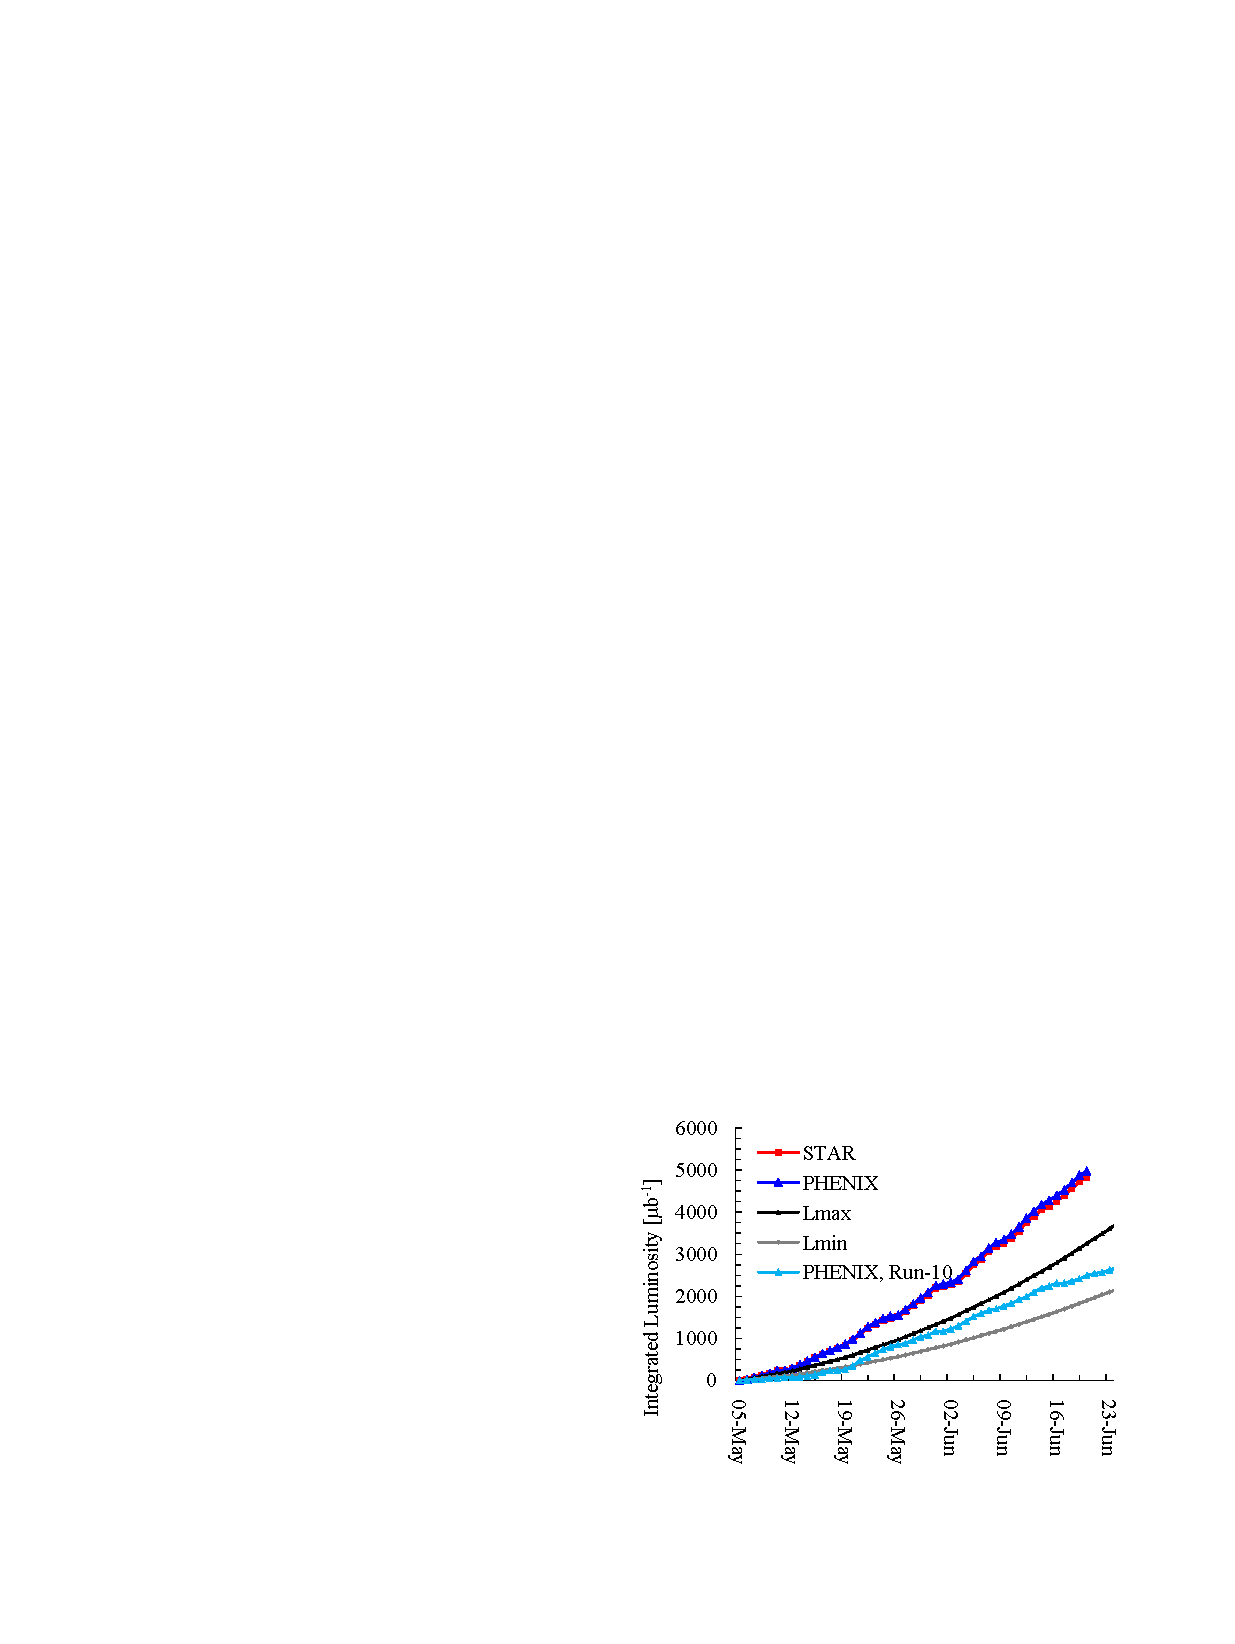
\includegraphics[width=\textwidth]{Plots/NPE/Run11_Lum.pdf}
        \caption{Run 11 Au+Au Integrated Luminosity}
        \label{fig:Luma}
    \end{subfigure}
    \begin{subfigure}{0.5\textwidth}
        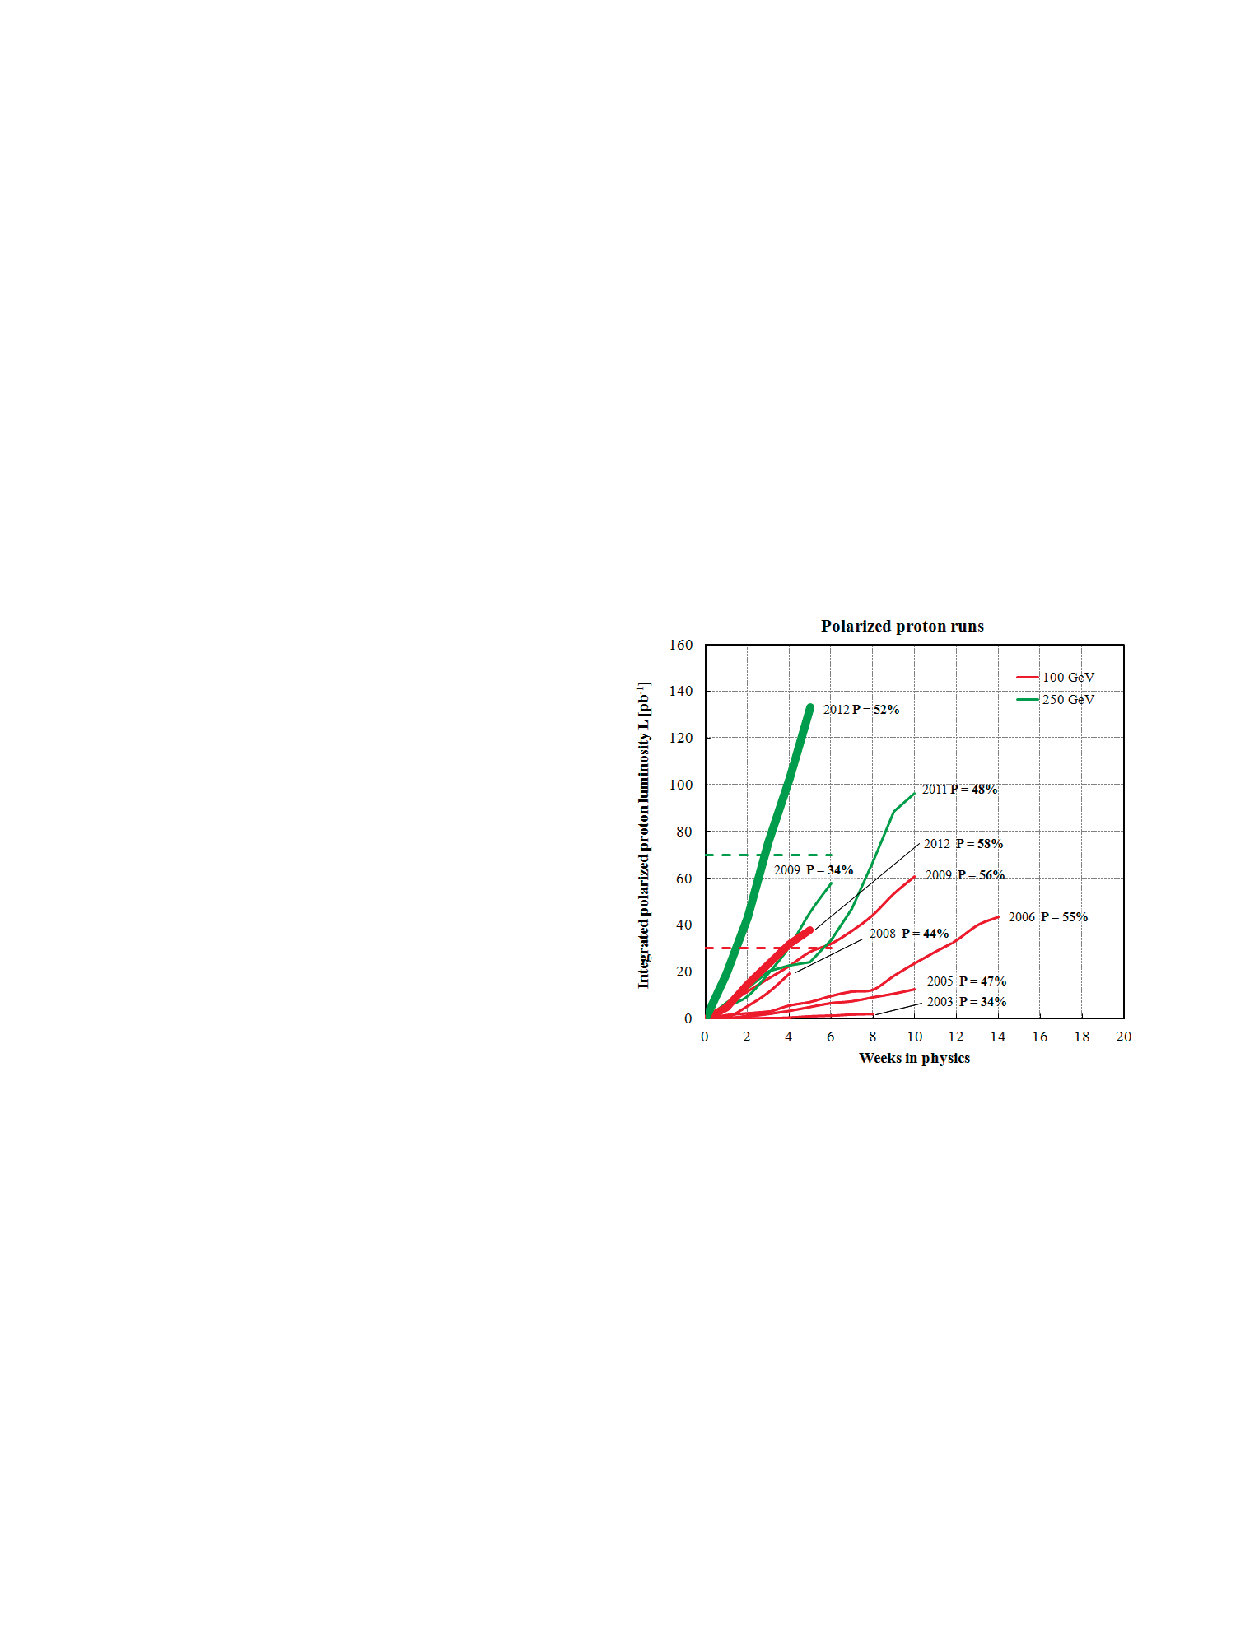
\includegraphics[width=\textwidth]{Plots/NPE/Run12_Lum.pdf}
        \caption{Run 12 p+p Integrated Luminosity}
        \label{fig:Lumb}
    \end{subfigure}
\caption[RHIC Integrated Luminosities in Run11 and Run12]{Integrated luminosities for run 11 and run 12 in RHIC. Left plot shows Au+Au delivered to STAR and PHENIX as well as run 10 in PHENIX for comparison. Right plot shows all p+p runs, run 12 is shown with thick lines.}
\label{fig:RunLum}
\end{figure}

The STAR data acquisition system handles several different triggers the most commonly used is the minimum bias trigger (minbias) which fires based on the coincidence of the STAR vertex position detector(VPD) and Zero Degree Calorimeters (ZDC) these events are prescaled so that only a fixed fraction of triggers are accepted so that the DAQ's data taking rate is not exceeded. STAR can also trigger on hits in the barrel EMC, these are the high tower (HT) triggers. A high tower trigger requires that a hit in a BEMC tower exceeds an ADC threshold determined such that the transverse energy in that tower is high. In run 11 we use the HT triggers NPE11, NPE15, NPE18, and NPE25 which are in increasing order of $E_{T}$. The NPE11 and NPE15 triggers are also prescaled. In p+p we use the BHT0, BHT1, BHT2, and BHT3 triggers, of these only BHT0 is prescaled.

Due to the large dataset sizes it is in our best interest to cut down on the data we need whenever possible. We do this first when we read the data to make BEMC points to match to tracks. Here we look through the tracks in the event and search for electron candidates based on the TPC information only. We throw out events without viable electron candidates. Since these cuts are looser than the electron cuts we will apply later we don't remove events we might actually want and we retain the ability to tighten the cuts later if we need to. After limiting ourselves to high tower triggers and keeping only events with electron candidates we are left with approximately 23 million events in Au+Au and 1.1 million events in p+p.

\subsection{Event Level Cuts}

At the event level we cut on events with vertex too far out of the center of the detector. We use the tracks in the TPC to reconstruct the vertex, we can also measure the vertex with the Vertex Position Detector (VPD). By convention we have the $x$ and $y$ axes as transverse to the beam line. The $z$ axis then runs along the beam. We require that the vertex be no more than 2 cm from the center of the beam pipe in the radial direction, i.e. $\sqrt{(V_x^{TPC})^2 + (V_y^{TPC})^2} \leq$ 2 cm. We also cut on the TPC vertex in the $z$ direction, choosing events with $|V_z^{TPC}| \leq$ 30 cm in Au+Au collisions and $|V_z^{TPC}| \leq$ 40 cm in p+p. Additionally we want to have good agreement between the vertices as measured by the TPC and VPD. We require that the difference between the measured $V_z$ satisfies $|V_z^{TPC} - V_z^{VPD} \leq|$ 4 cm in Au+Au. Figure~\ref{fig:Vertexz} shows the distribution of $V_z^{TPC}$ and the difference in TPC and VPD $V_z$ in Au+Au collisions. In p+p because of lower multiplicity and a wider vertex distribution the measured vertex from VPD is not reliable and thus the cut on the difference of $V_z$ is not used.

\begin{table}
\centering
\begin{tabular}{|c|c|}
\hline
Variable            & Cut \\
\hline
Triggers (Au+Au)          & NPE11 NPE15 NPE18 NPE25 \\
\hline
Triggers (p+p)          & BHT0 BHT1 BHT2 BHT3 \\
\hline
$|V_z^{TPC}|$  (Au+Au)        & $\leq$ 30 cm \\
\hline
$|V_z^{TPC}|$  (p+p)        & $\leq$ 40 cm \\
\hline
$|V_z^{TPC} - V_z^{ZDC}|$  (Au+Au only)        & $\leq$ 4 cm \\
\hline
\end{tabular}
\caption[Dataset and Event Level Cuts]{Datasets used in the analysis as well as the cuts applied at the event level.}
\label{tab:TPCQual}
\end{table}

\begin{figure}[htbp]
    \begin{subfigure}{0.5\textwidth}
        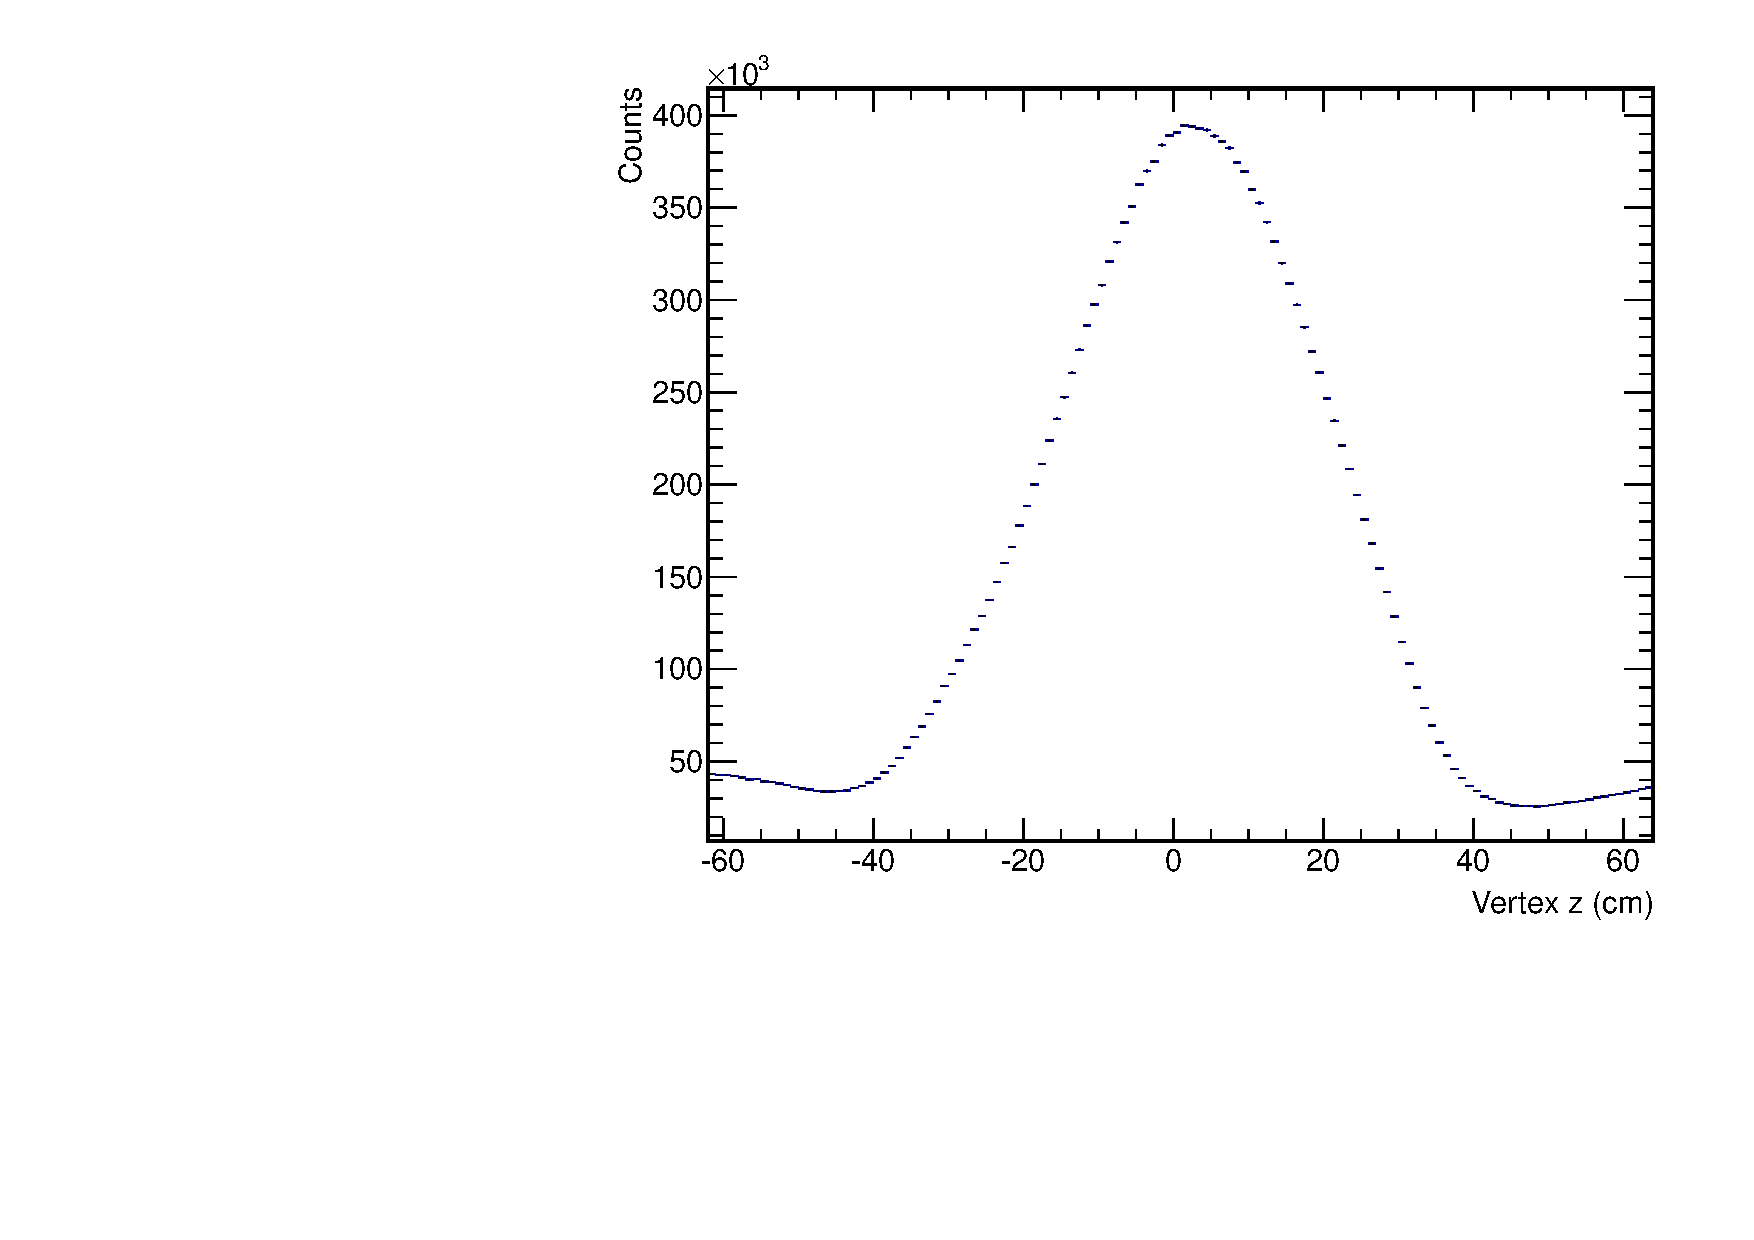
\includegraphics[width=\textwidth]{Plots/NPE/VzAuAu.pdf}
        \caption{$V_{z}^{TPC}$}
        \label{fig:VzAuAu}
    \end{subfigure}
    \begin{subfigure}{0.5\textwidth}
        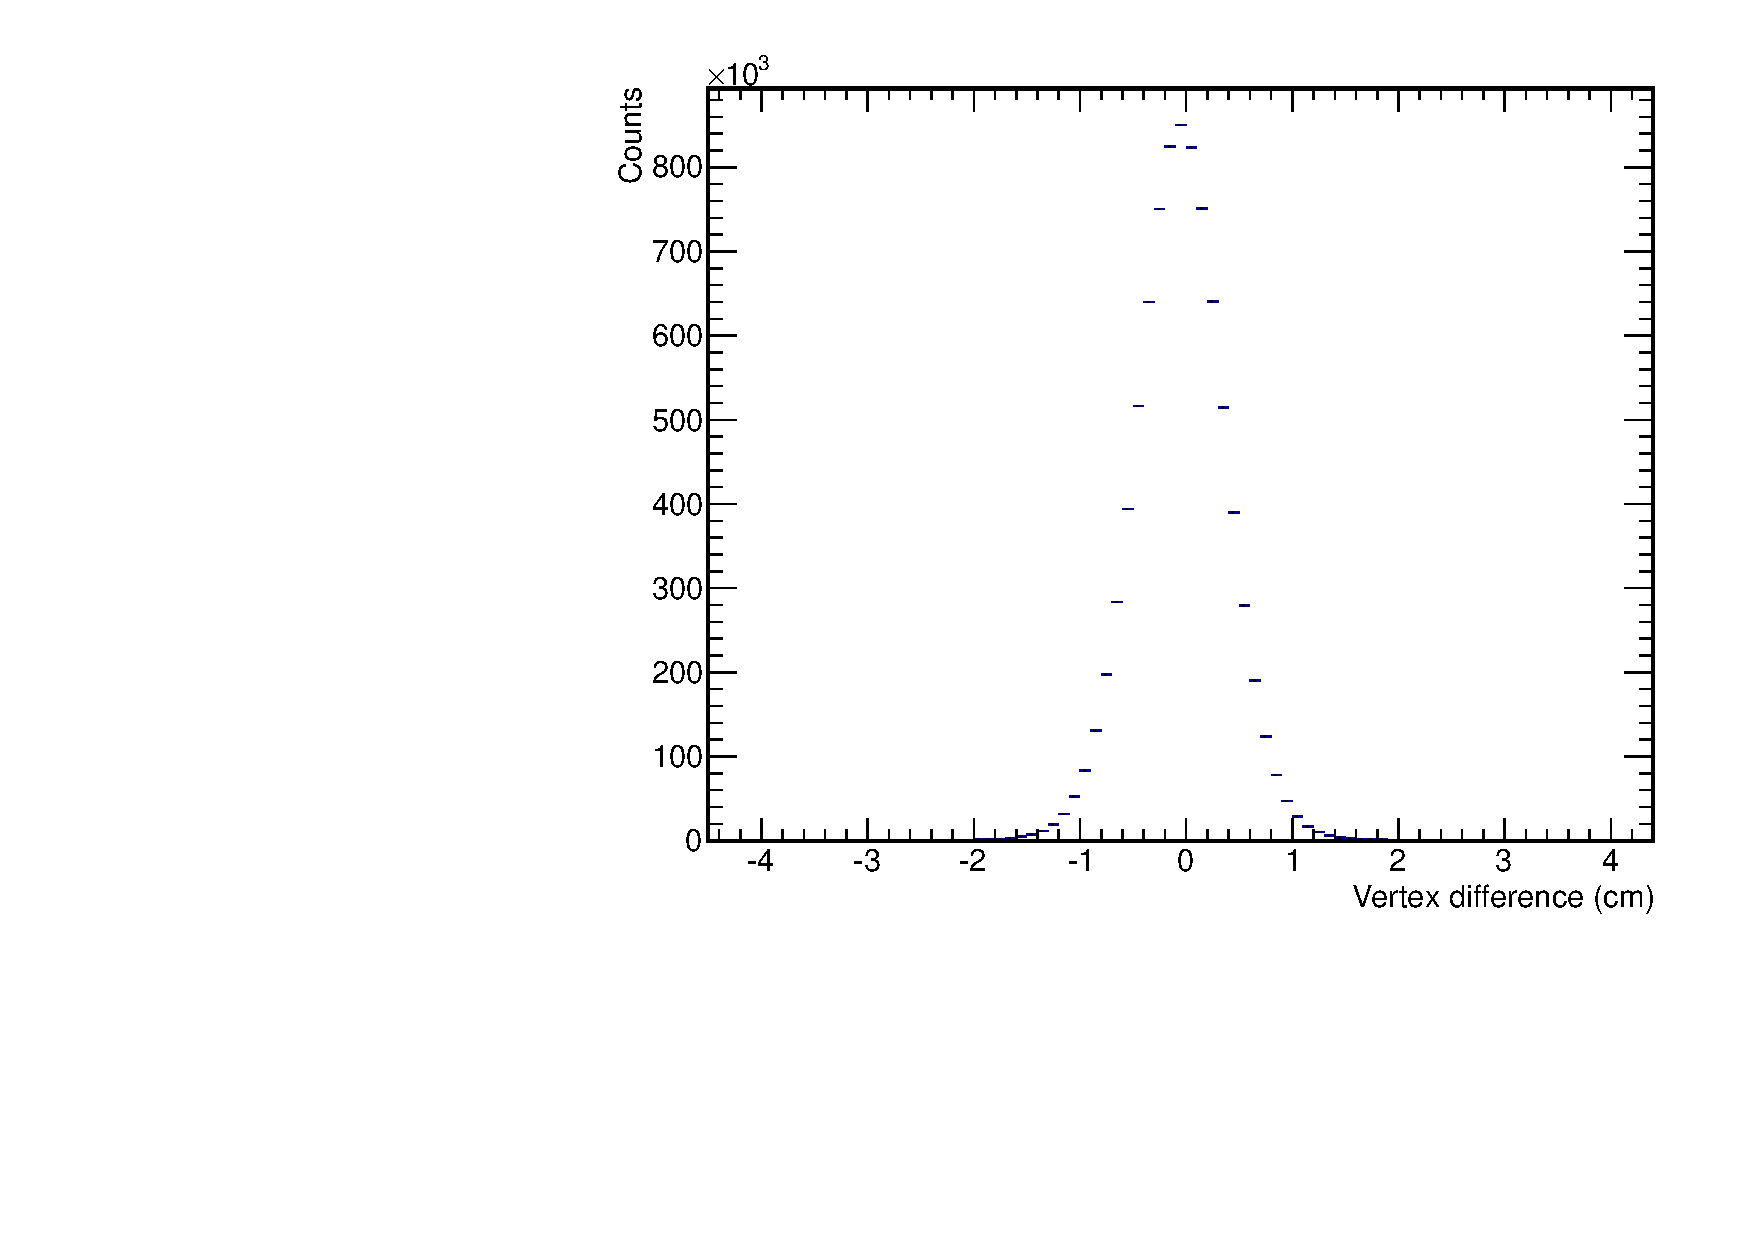
\includegraphics[width=\textwidth]{Plots/NPE/VzDiff.pdf}
        \caption{$V_z^{TPC} - V_z^{VPD}$}
        \label{fig:VertexDiff}
    \end{subfigure}
\caption[TPC $V_z$ and TPC VPD Difference]{Vertex z distribution in run 11 Au+Au. Left plot shows the distribution of the z vertex (cut at $\pm$30 cm), right plot shows the difference between TPC and VPD $V_z$ (cut at $\pm$4 cm).}
\label{fig:Vertexz}
\end{figure}

At the event level we also determine the centrality using the STAR \texttt{StRefMultCorr} class which calculates the centrality bin based on the reference multiplicity (refmult), vertex z, run number, and ZDC coincidence rate. Figure~\ref{fig:EventCent} shows the event by event distribution of refmult as well as the number of events from each centrality bin used in the NPE analysis.
 
\begin{figure}[htbp]
    \begin{subfigure}{0.5\textwidth}
        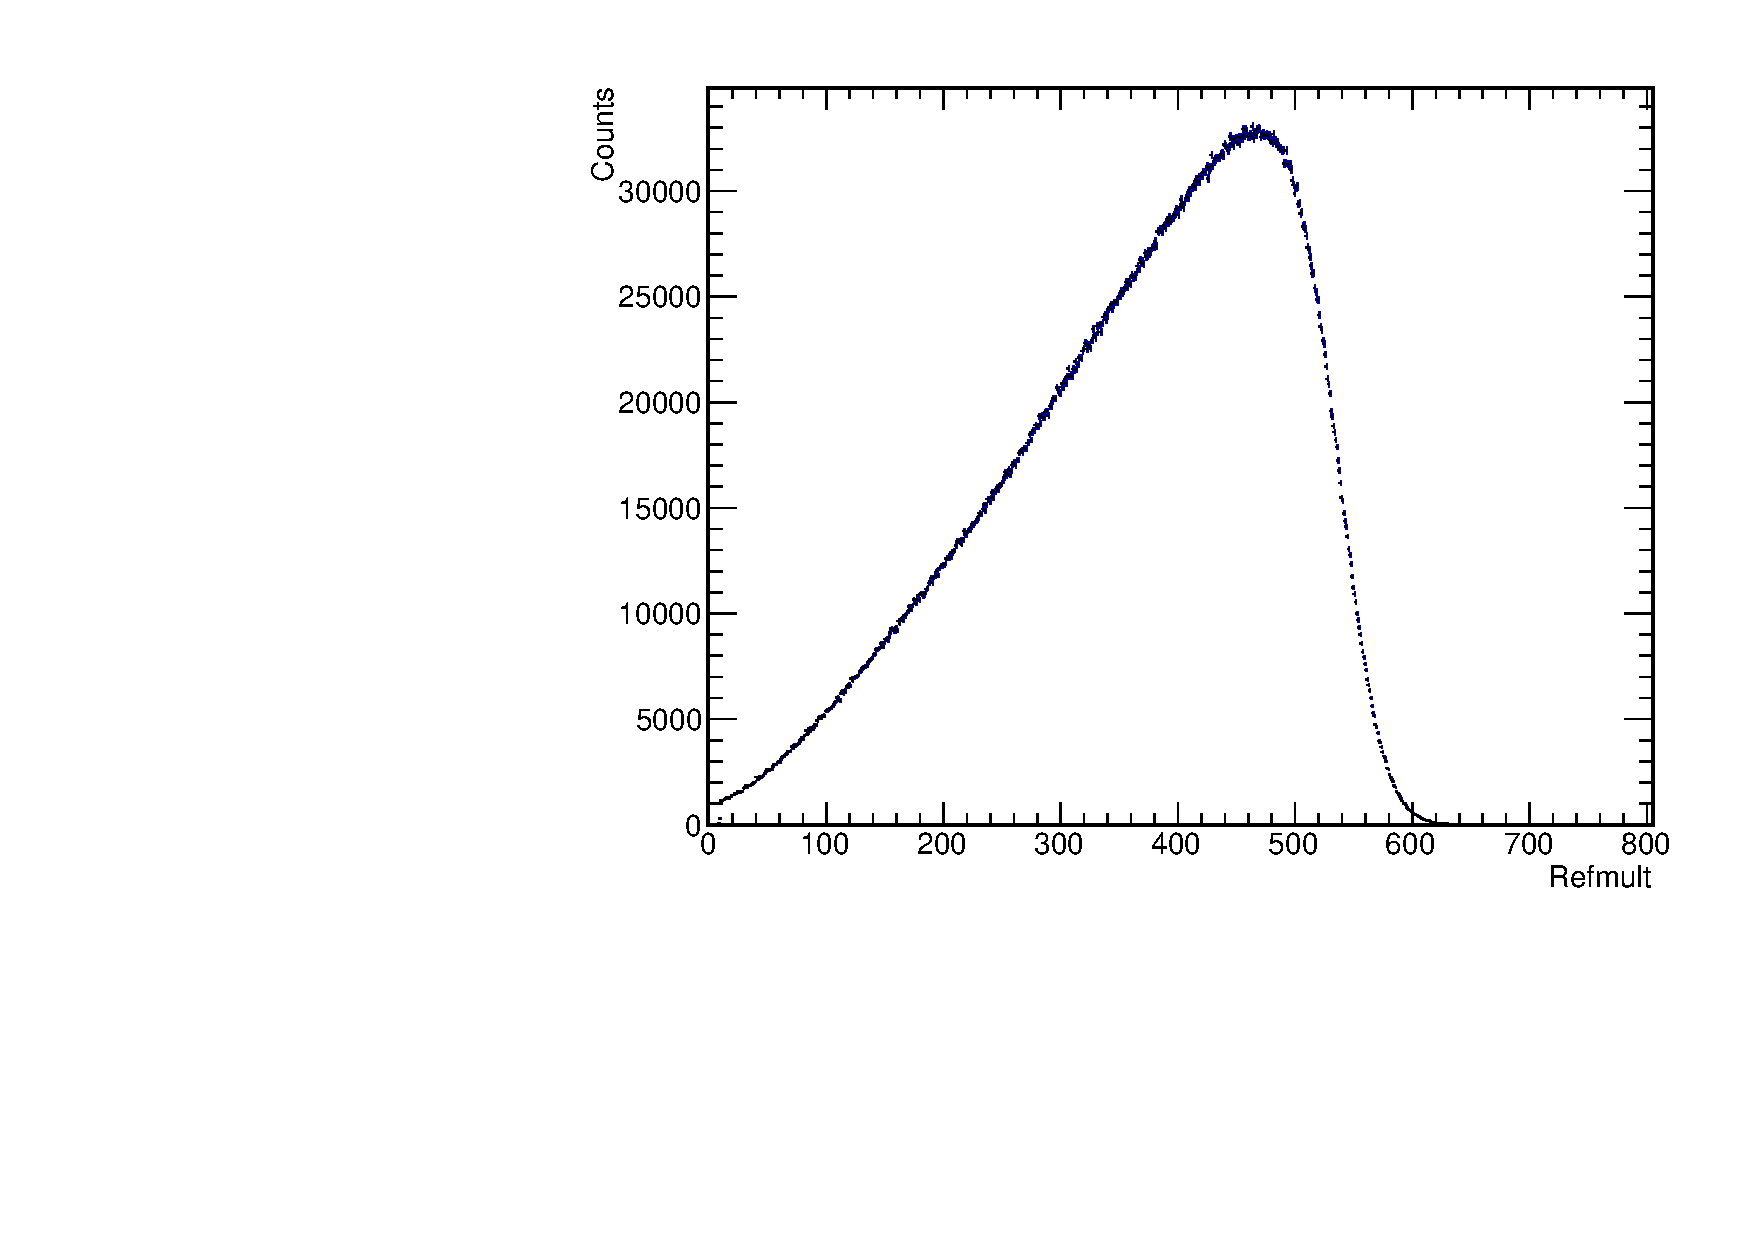
\includegraphics[width=\textwidth]{Plots/NPE/RefmultNPE18.pdf}
        \caption{Reference Multiplicity}
        \label{fig:refmult}
    \end{subfigure}
    \begin{subfigure}{0.5\textwidth}
        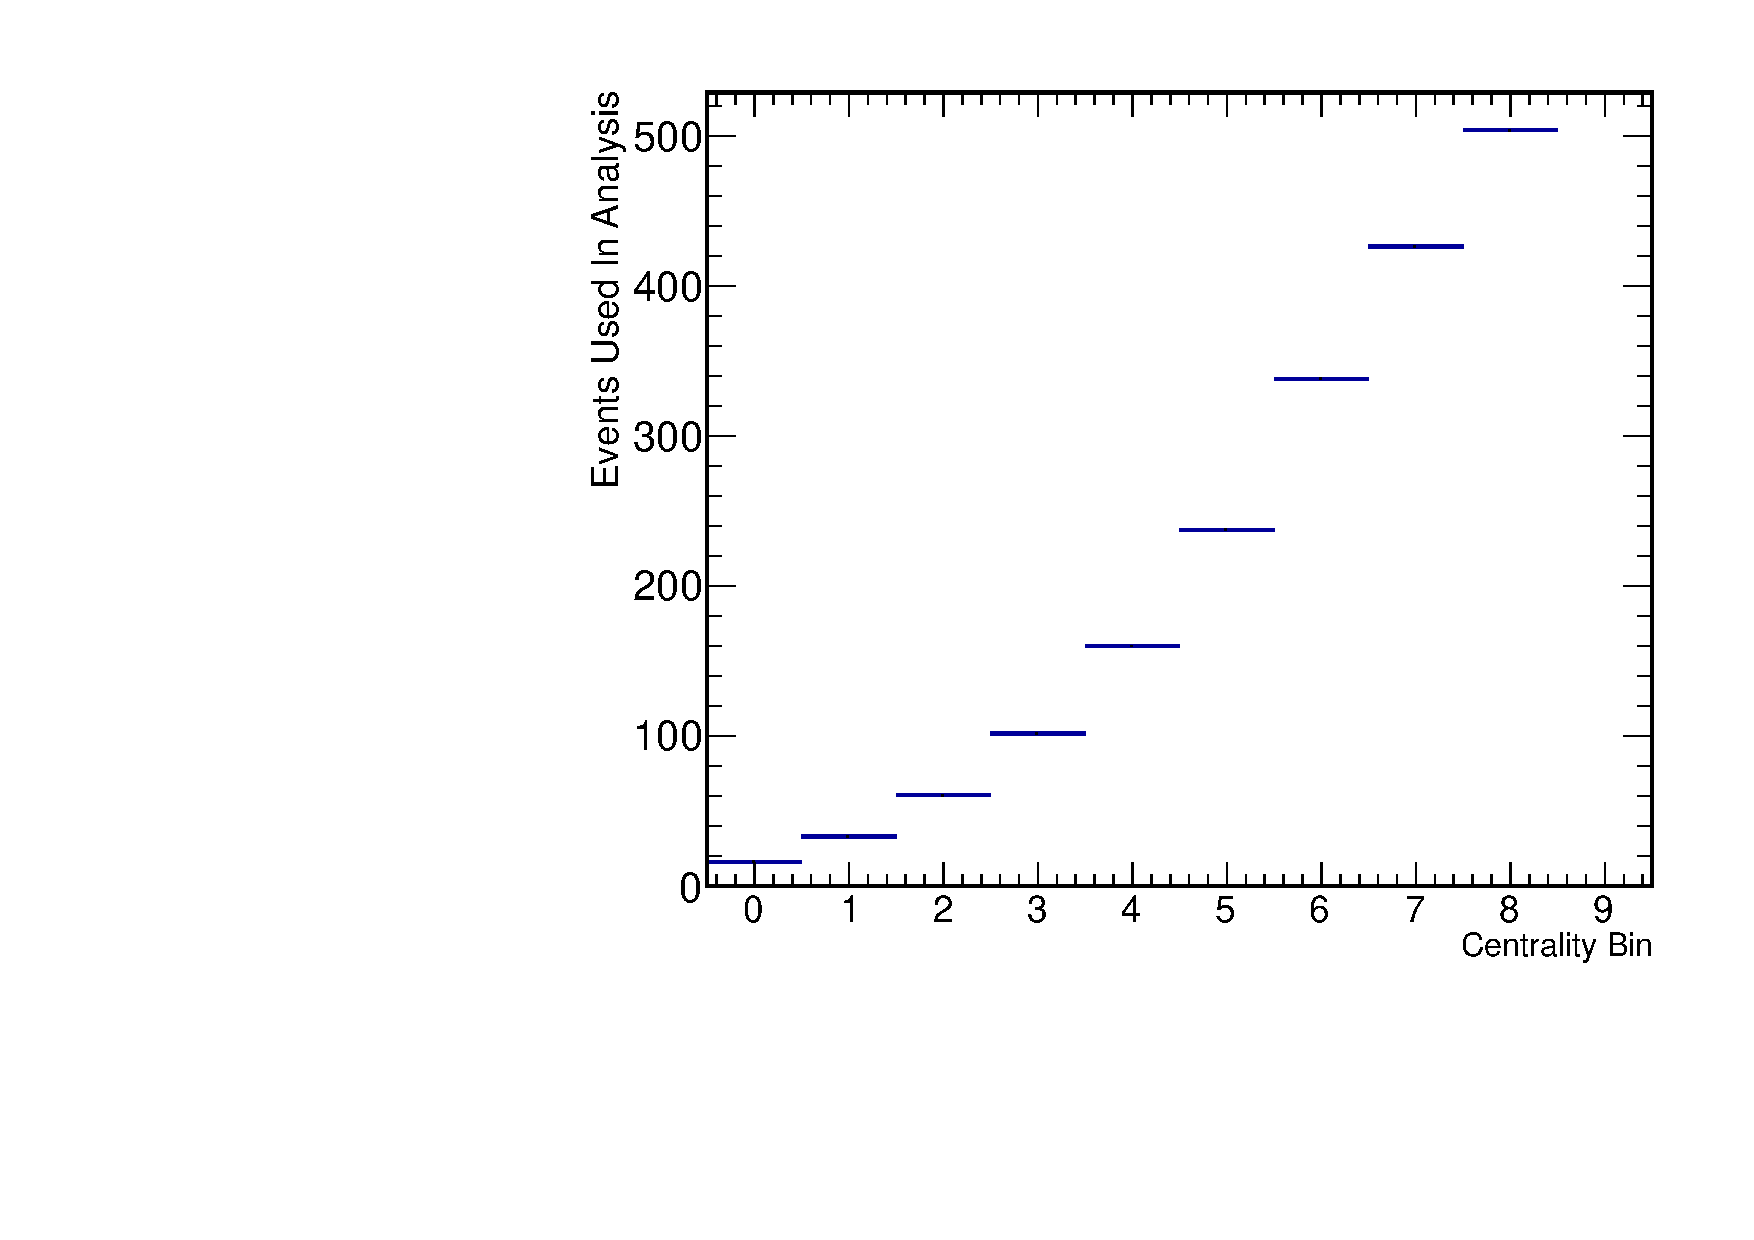
\includegraphics[width=\textwidth]{Plots/NPE/Centrality_dist.pdf}
        \caption{Centrality bins}
        \label{fig:centdist}
    \end{subfigure}
\caption[Refmult and Centrality Distributions]{Reference multiplicity and centrality bin distributions for HT trigger events in Au+Au.}
\label{fig:EventCent}
\end{figure}

\section{Track Reconstruction and TPC Cuts}

The TPC is the primary tracking and particle identification system in STAR. Charged particles traverse the TPC chamber which ionizes the gas inside. Due to the nearly uniform electric field in the TPC these ions drift to the ends of the TPC where the currents are read out by the TPC padrows. The magnetic field in the TPC causes charged particle trajectories to be helical making charge sign distinction possible. We can also use the TPC for particle identification by measuring the ionization energy loss in the detector. 

In the TPC we consider two types of tracks. The global tracks are those tracks from the fit to hits inside the TPC. If a global track has a distance of closest approach (DCA) to the primary vertex less than 3 cm then the primary vertex is added to the track hits and the track is refit. The resulting track is a primary track, which should represent particles coming directly from the collision.

We impose track quality cuts to make sure the track fits are good and that we get a good measurement of $dE/dx$. For primary tracks we require the number of TPC hits used in the track fit is between 20 and 50. For global tracks we only require that the number of hits is above 15. For all tracks we also cut on the ratio of hits fit to the maximum number possible keeping it between .52 and 1.05.

In run 11 and run 12 we have no tracking information near the beam pipe, the Silicon Vertex Tracker was removed before the runs and the new Heavy Flavor Tracker had not been installed. Due to the relatively short decay length (~100 $\mu$m) of $D$ and $B$ mesons this means that the decay vertex of these particles can not be distinguished from the primary vertex. For electron candidates we require primary tracks with DCA of less than 2 cm. The corresponding global track for that electron must also be less than 3 cm. 

\begin{table}
\centering
\begin{tabular}{|c|c|}
\hline
Variable            & Cut \\
\hline
TPC Hits (Primary Tracks)          & $\in(20, 50)$ \\
\hline
TPC Hits (Global Tracks)          & $\geq 15$ \\
\hline
$N_{\text{hits}}/N_{\text{possible}}$               & $\in(.52, 1.05)$ \\
\hline
Primary DCA          & $< 2.0$cm \\
\hline
\end{tabular}
\caption[Track Quality Cuts]{Quality cuts used for TPC tracks.}
\label{tab:TPCQual}
\end{table}

The energy loss ($dE/dx$) in the TPC is modeled by the Bichsel function which also accounts for the spread in values for different particle species. We will be looking at the deviation of the energy loss compared to the Bichsel function value for electrons. This quantity is called $n\sigma_e$ and is defined as:

\begin{equation}\label{eq:nsigmae}
n\sigma_e = \frac{\log{\frac{dE/dx}{B_e}}}{\sigma_e}
\end{equation}

where $B_e$ is the Bichsel function value and $n\sigma_e$ is the deviation from the mean Bichsel function value for electrons. Analagous values are defined for protons, kaons, and pions but we will only concern ourselves with $n\sigma_e$. We will go over the specific $n\sigma_e$ cuts used when we discuss the details of electron identification. 

\section{BEMC Points and Matching}

The BEMC is critical to the identification of high $p_T$ electrons in STAR. In Au+Au and p+p collisions hadrons (mostly pions and protons) greatly outnumber electrons and the $n\sigma_e$ cuts in the TPC are not enough to give an acceptable electron purity. With the BEMC electron identification is possible at high $\pt$, in the calorimeter electrons are much more likely to interact in the first few layers of the calorimeter and they will also deposit their entire energy within the tower. 

The barrel information in an event gives us hits for the BEMC towers as well as hits in the $\eta$ and $\phi$ directions for the shower max detector. From this information we need to cluster the tower hits as well as find hits in the SMD. Then we need to take the BEMC points (tower cluster and SMD hits) and associate it with a track from the TPC. We want to cluster the tower and SMD hits such that each BEMC point is associated with one electron. With the combined TPC and BEMC information we can identify the high $\pt$ electrons necessary for our analysis.

We will now describe the UCLA BEMC point making program and will use the following definitions: 

\begin{itemize}
\item \textbf{Tower cluster:} Group of tower hits according to some clustering criterion.
\item \textbf{BSMD hit:} Signal in a single strip in the BSMD in either $\phi$ or $\eta$.
\item \textbf{BSMD cluster:} Group of BSMD hits in either $\phi$ or $\eta$.
\item \textbf{BSMD point:} Pair of clusters, one from $\phi$, the other $\eta$, which give a spatial point on the detector.
\item \textbf{BEMC point:} A tower cluster and an associated BSMD point which will be matched up with tracks from the TPC.
\end{itemize}

To use the UCLA EMC point maker, described in detail in ref, to construct points and associate them with TPC tracks. The first step in reconstructing the BEMC points is to find and cluster the hits in the BEMC towers. To do this we first look for seed towers which have deposited energy above .1 GeV/c. Once we have found a seed tower adjoining towers within the same BEMC module are clustered with the seed, there is no clustering of towers or SMD hits across the modules. 

The BSMD uses a similar clustering procedure for both the $\phi$ and $\eta$ directions. If EMC towers and BSMD clusters are found then the program will check for multiple clusters and attempt to merge them by relaxing the SMD clustering criteria. If one direction in the BSMD has no hits then clustering is rerun with relaxed criteria to try and find a good SMD point for that module. If neither tower nor SMD clusters are found in a module then the algorithm moves on to the next module. 

With clusters in the towers and possibly the SMD found we move on to asscociating tower clusters to SMD hits. We only use SMD hits adjacent to the tower cluster and if there is only one SMD point associate it with the cluster. For the case of multple SMD hits adjacent to the tower the tower energy is divided between the SMD points. If there are no points in the SMD but we still have tower clusters then the tower cluster is kept but not used as a BEMC point for matching with the TPC. The SMD info is used as the $\phi$ and $\eta$ location of the hit and the tower cluster is used for the point's energy. Figure~\ref{fig:SMDetaphi} shows the distribution of SMD points in $\phi$ and $\eta$.

\begin{figure}[htbp]
\begin{center}
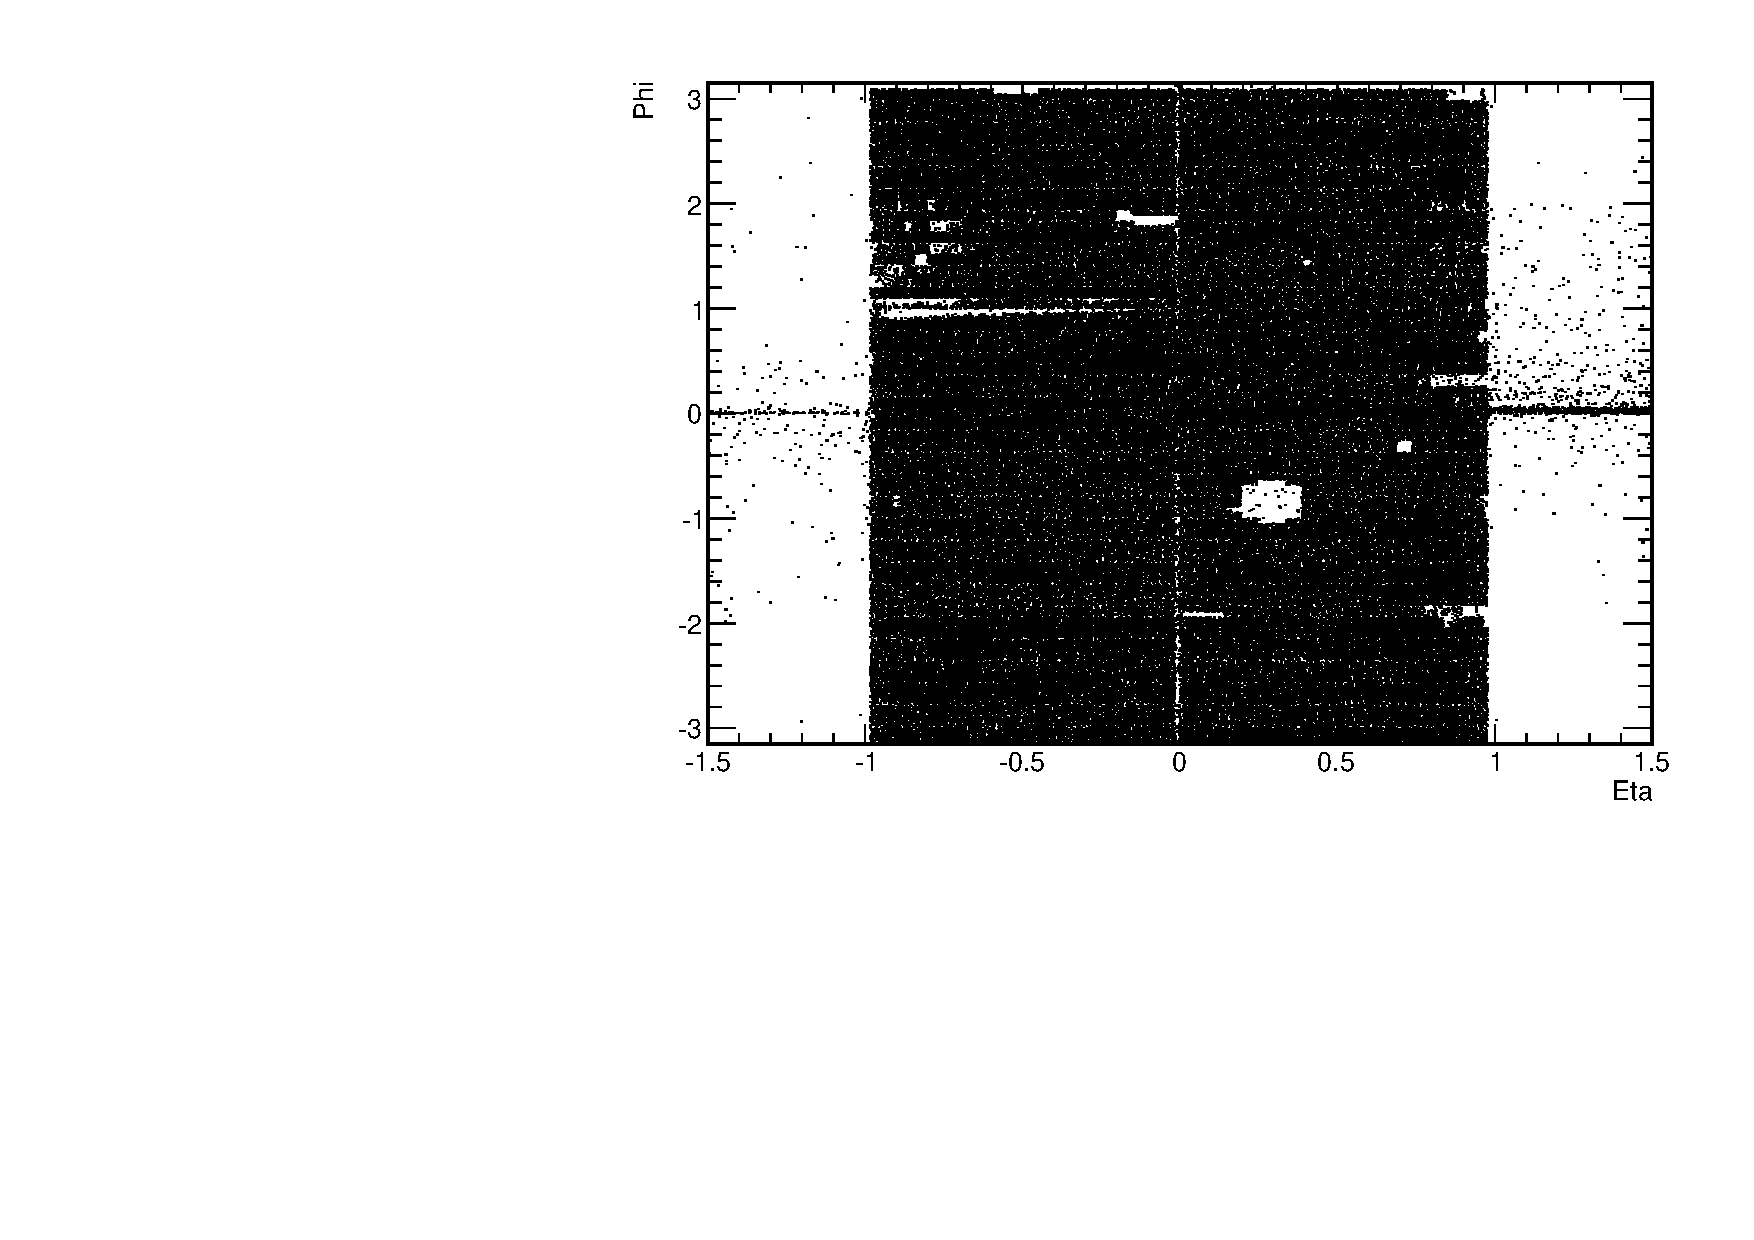
\includegraphics[scale=.8]{Plots/NPE/SMD_phi_eta.pdf}
\end{center}
\caption[SMD Point $\eta$ and $\phi$]{SMD points in $\eta$ and $\phi$ for the EMC points used in the analysis}
\label{fig:SMDetaphi}
\end{figure}

From the TPC we only consider tracks with $\pt$ above 1.5 GeV/c for association with points in the BEMC. When the TPC tracks are reconstructed they are fit to a helix to describe their trajectory through the TPC magnetic field. We then project these helices to the inner surface of the BEMC. After the projection we then associate the track with a BEMC point. We require that the distance between the points ($d = \sqrt{\Delta\phi^2 + \Delta\eta^2}$) be smaller than .05. If multiple BEMC points are close enough to be matched, then we select the one with the smallest distance. In general tracks from electrons will match better to the points in the BEMC, we will use this to improve the cuts for electron identification which will be discussed in the next section.

\section{Electron Identification}

We can now use the matched TPC tracks and BEMC points to identify electrons in Au+Au and p+p collisions. We will use the TPC information to find tracks that originate from the primary vertex, traverse the TPC depositing energy consistent with what we would expect from electrons, then interact in the first few layers of the BEMC leaving a wide shower that terminates within the tower.

\subsection{BEMC Cuts}

Our analysis only uses data from high tower trigger events. The only requirement for a high tower trigger is that a tower in the event register a hit above a certain threshold. There is no guarantee that the tower will be matched to a track or that an electron triggered the tower. However we may still find electrons in these events they will just be below the trigger threshold. This effect is called random trigger benefit and it is important to remove in NPE analyses where the production cross-section of NPE is important. It is likely not critical in this analysis because we will be looking at correlations which are normalized per trigger but we still attempt to cut out the random trigger benefit. 

When we make the BEMC points we also record the highest tower ADC value in the BEMC cluster and record this as the ADC0 for that point. Figure~\ref{fig:ADC0} shows the distribution of ADC0 from primary tracks matched to BEMC points. Near 325 ADC counts we see a large rise in the ADC0 of points, this corresponds to the threshold for the NPE18 trigger. Any electrons with ADC0 much below this value can be assumed to come from random trigger benefits and are not used. 

\begin{figure}[htbp]
\begin{center}
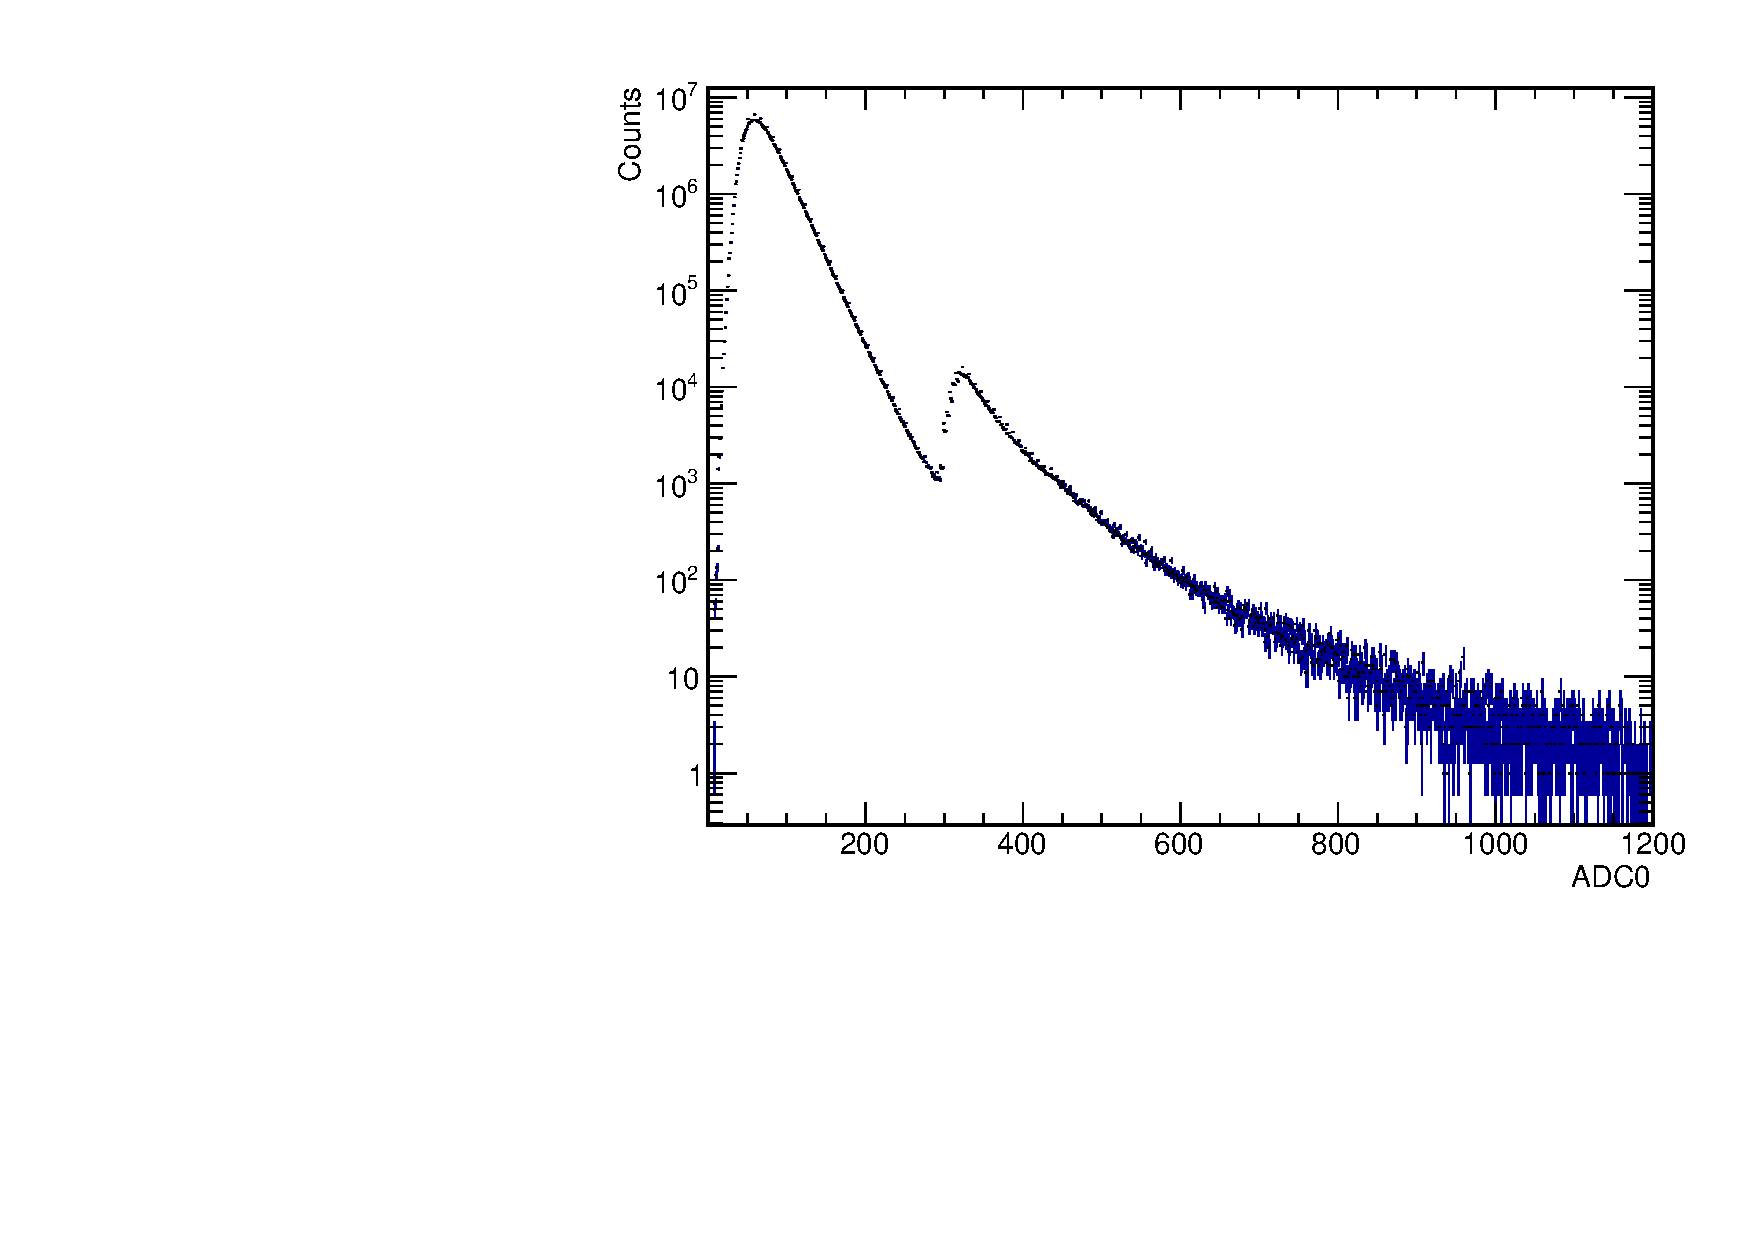
\includegraphics[scale=.8]{Plots/NPE/ADC0_NPE18.pdf}
\end{center}
\caption[ADC0 Distribution for NPE18]{ADC0 for primary tracks in NPE18 triggered events. Turn on of the NPE18 trigger is apparent around 325 ADC counts.}
\label{fig:ADC0}
\end{figure}

For NPE, due to the short lifetime of the parent mesons, we only consider tracks originating from the primary vertex. Further we cut on the DCA of the track to the primary vertex, requiring that that the DCA be less than 1.5 cm. This cut is tighter than the 2 cm cut we used when considering the TPC track quality. We also remove tracks with $p_T$ < 2.0 GeV/c, generally the tracks comming from triggered electrons will be much higher than this anyway. For our acceptance we want the electron to be -.7 $\leq \eta \leq$ .7 in  pseudorapidity. This corresponds to the $\eta$ acceptance of the BEMC. Run 10 analyses also cut out areas in $\phi$ which correspond to the position of the SVT support structure. The reasoning behind that cut is that the remaining structure could cause more photon conversions in those regions, but this cut is not applied here.

Now we apply the BEMC information to select electrons. Electrons begin showering much earlier in the BEMC than hadrons, the SMD sits at $5.6 X_0$ where electromagnetic showers are widest. With more hits in the SMD the spatial resolution of the BEMC points is better as so the BEMC matching for electrons tends to be better. This is illustrated in Figures~\ref{fig:point_dphi} and~\ref{fig:dZ} which show the BEMC matching in $\Delta\phi$ and $\Delta Z$. Black points are for all matched primary tracks and red points show the matching for identified electrons (with the matching cuts excluded). We set the $\Delta\phi$ cut such that $|\Delta\phi| \leq$ .013 and for $\Delta Z$ we use -2.5 cm $\leq \Delta Z \leq$ 1.1 cm (for $\eta >$ 0) and -1.5 cm $\leq \Delta Z \leq$ 1.9 cm (for $\eta <$ 0). Figure~\ref{fig:dZ} different cuts on $\Delta Z$ are applied in the different halves of the TPC due to a discreet jump when crossing the central membrane of the TPC.

\begin{figure}[htbp]
\begin{center}
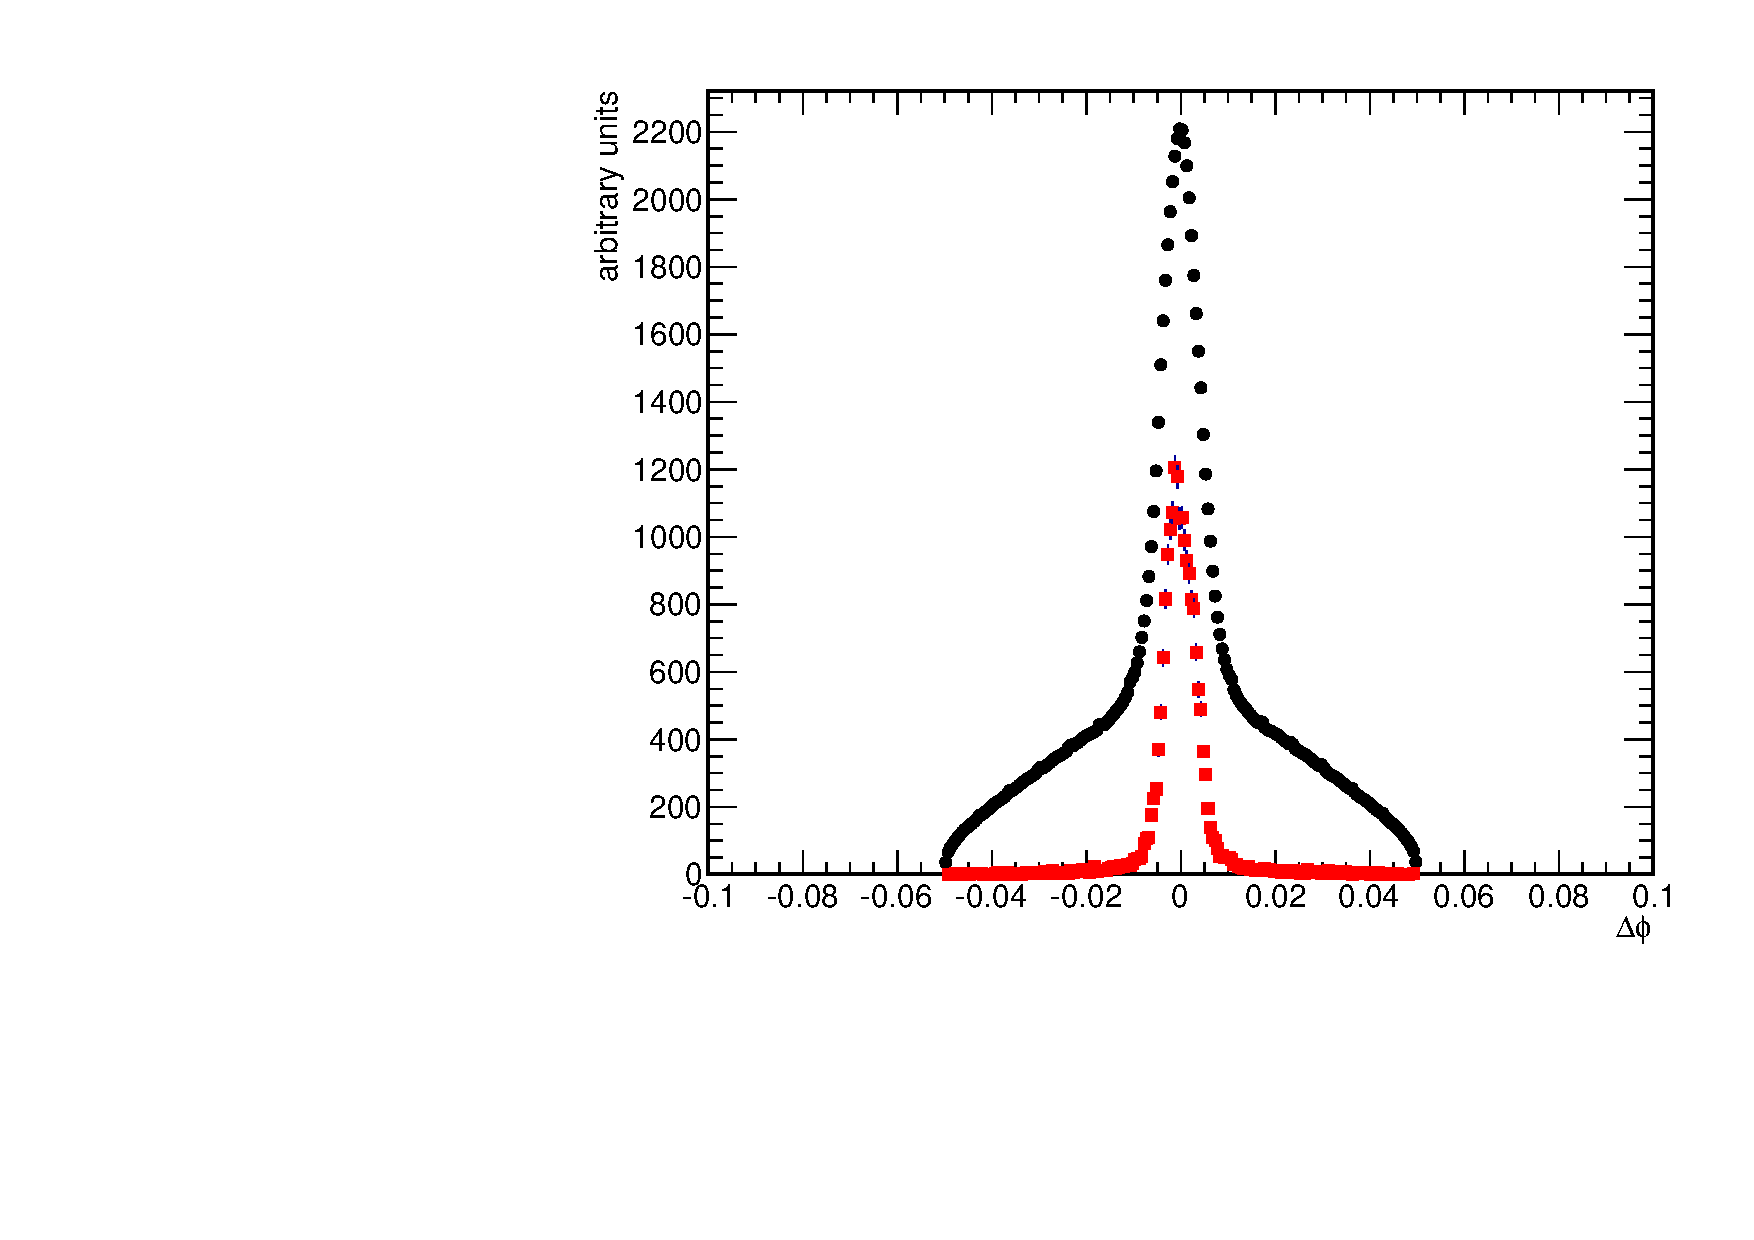
\includegraphics[scale=.8]{Plots/NPE/point_dphi.pdf}
\end{center}
\caption[TPC to BEMC $\Delta\phi$]{$\Delta\phi$ between the TPC and BEMC for all matched primary tracks (black) and identified electrons (red). Y-axis is arbitrary units scaled to show all tracks and electrons on the same figure. Matching is better for electrons and we cut on such that $|\Delta\phi| \leq$ .013.}
\label{fig:point_dphi}
\end{figure}

\begin{figure}[htbp]
	\begin{center}
    \begin{subfigure}{0.65\textwidth}
        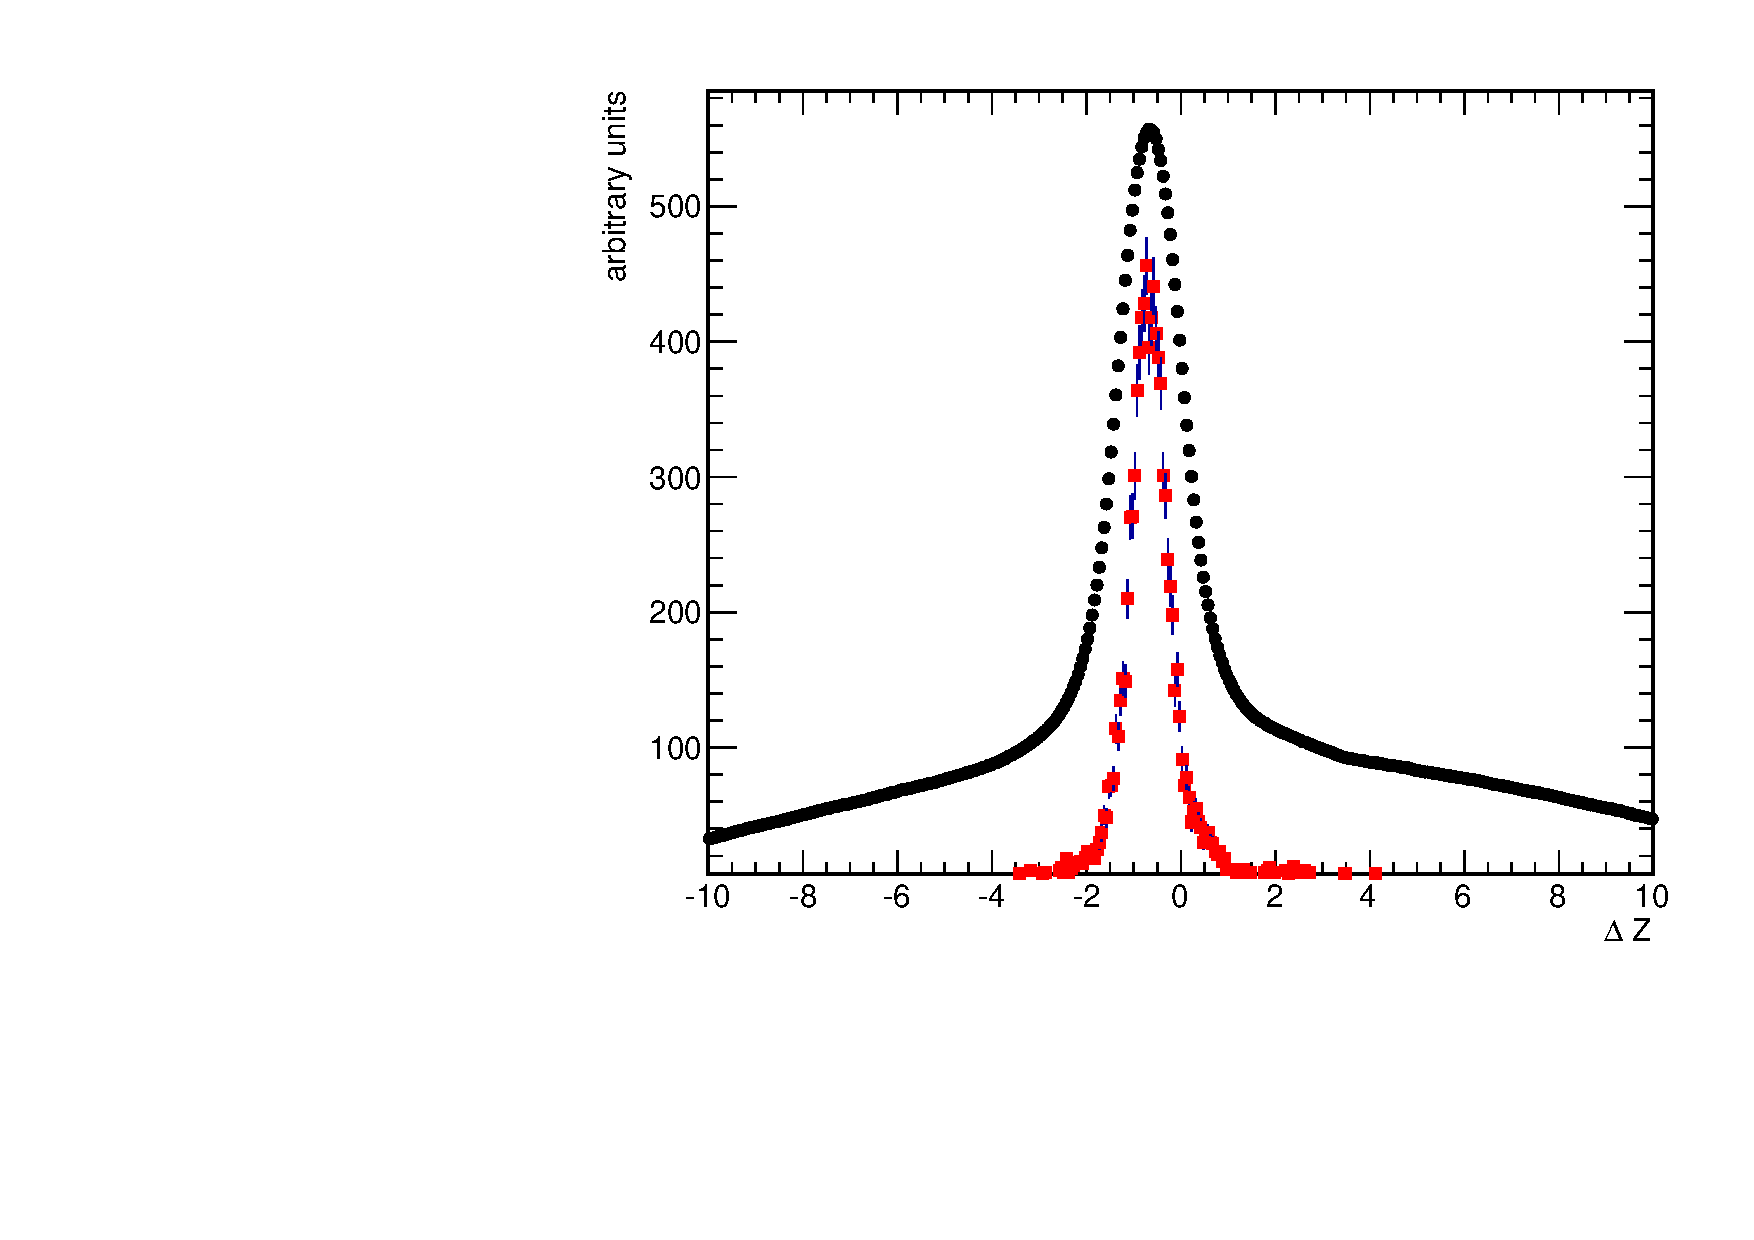
\includegraphics[width=\textwidth]{Plots/NPE/dZ_pos.pdf}
        \caption{$\eta >$ 0}
        \label{fig:dZpos}
    \end{subfigure}
    \begin{subfigure}{0.65\textwidth}
        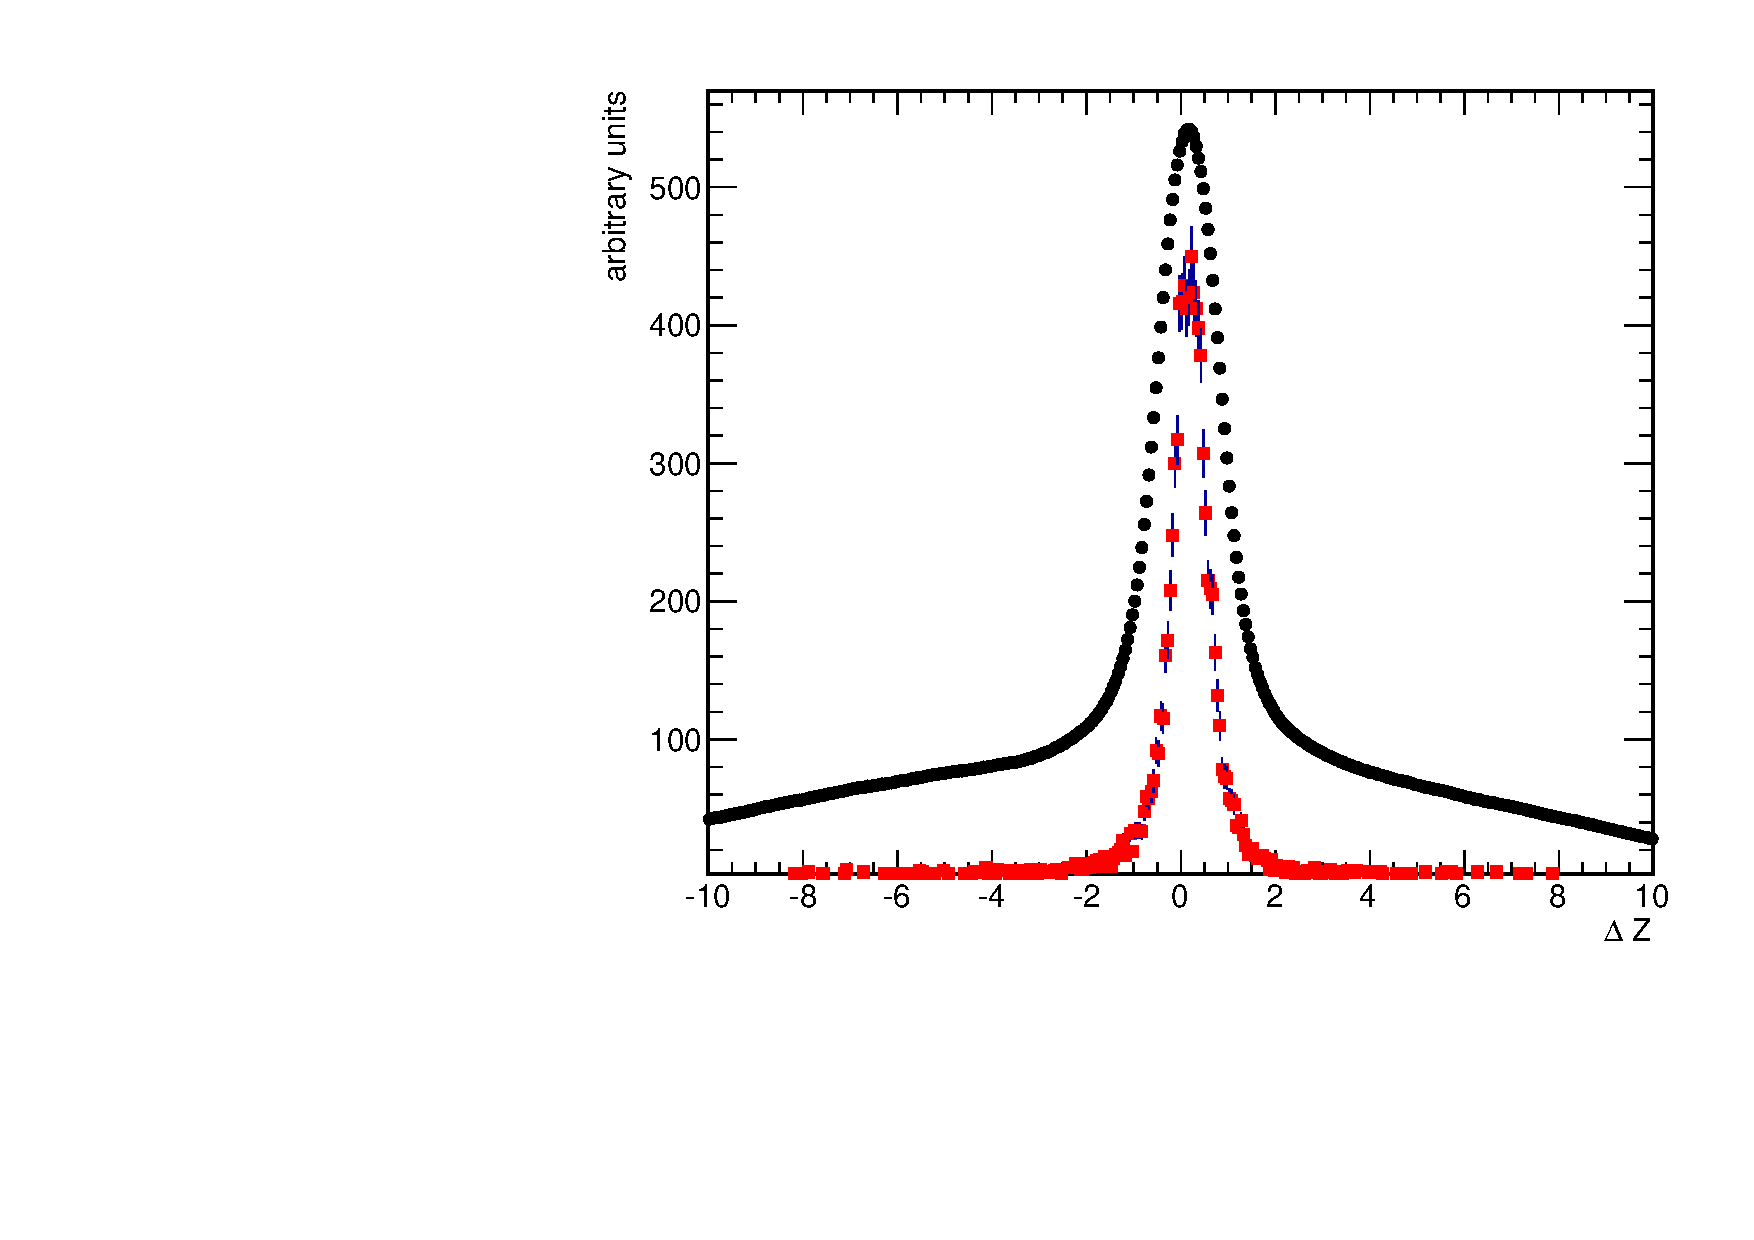
\includegraphics[width=\textwidth]{Plots/NPE/dZ_neg.pdf}
        \caption{$\eta <$ 0}
        \label{fig:dXneg}
    \end{subfigure}
	\end{center}
\caption[TPC to BEMC $\Delta Z$]{$\Delta Z$ of the TPC track to BEMC point for all points and for electrons. Different cuts are used in the two halves of the TPC due to a jump when moving from the positive $\eta$ region to negative.}
\label{fig:dZ}
\end{figure}

The wider showers for electrons also make it possible to cut on electrons based on the number of hits in the BSMD. The strips in the SMD are approximately twice the Moliere radius for electrons in lead, thus for developed EM showers we expect to see hits in multiple strips. Most hadrons will not leave hits in the BSMD, but since we are only considering reconstructed points in the BEMC we know that we will have at least one hit in both $\eta$ and $\phi$ in the SMD. Figure~\ref{fig:SMDstrips} shows the hits in the SMD for hadrons and for photonic electrons. We show the cuts with photonic electrons because without the SMD cuts the sample of BEMC points is not pure enough to illustrate the difference in behavior between hadrons and electrons. For electrons we require that number of strip hits in both $\phi$ and $\eta$ be greater than or equal to 2.

\begin{figure}[htbp]
	\begin{center}
    \begin{subfigure}{0.65\textwidth}
        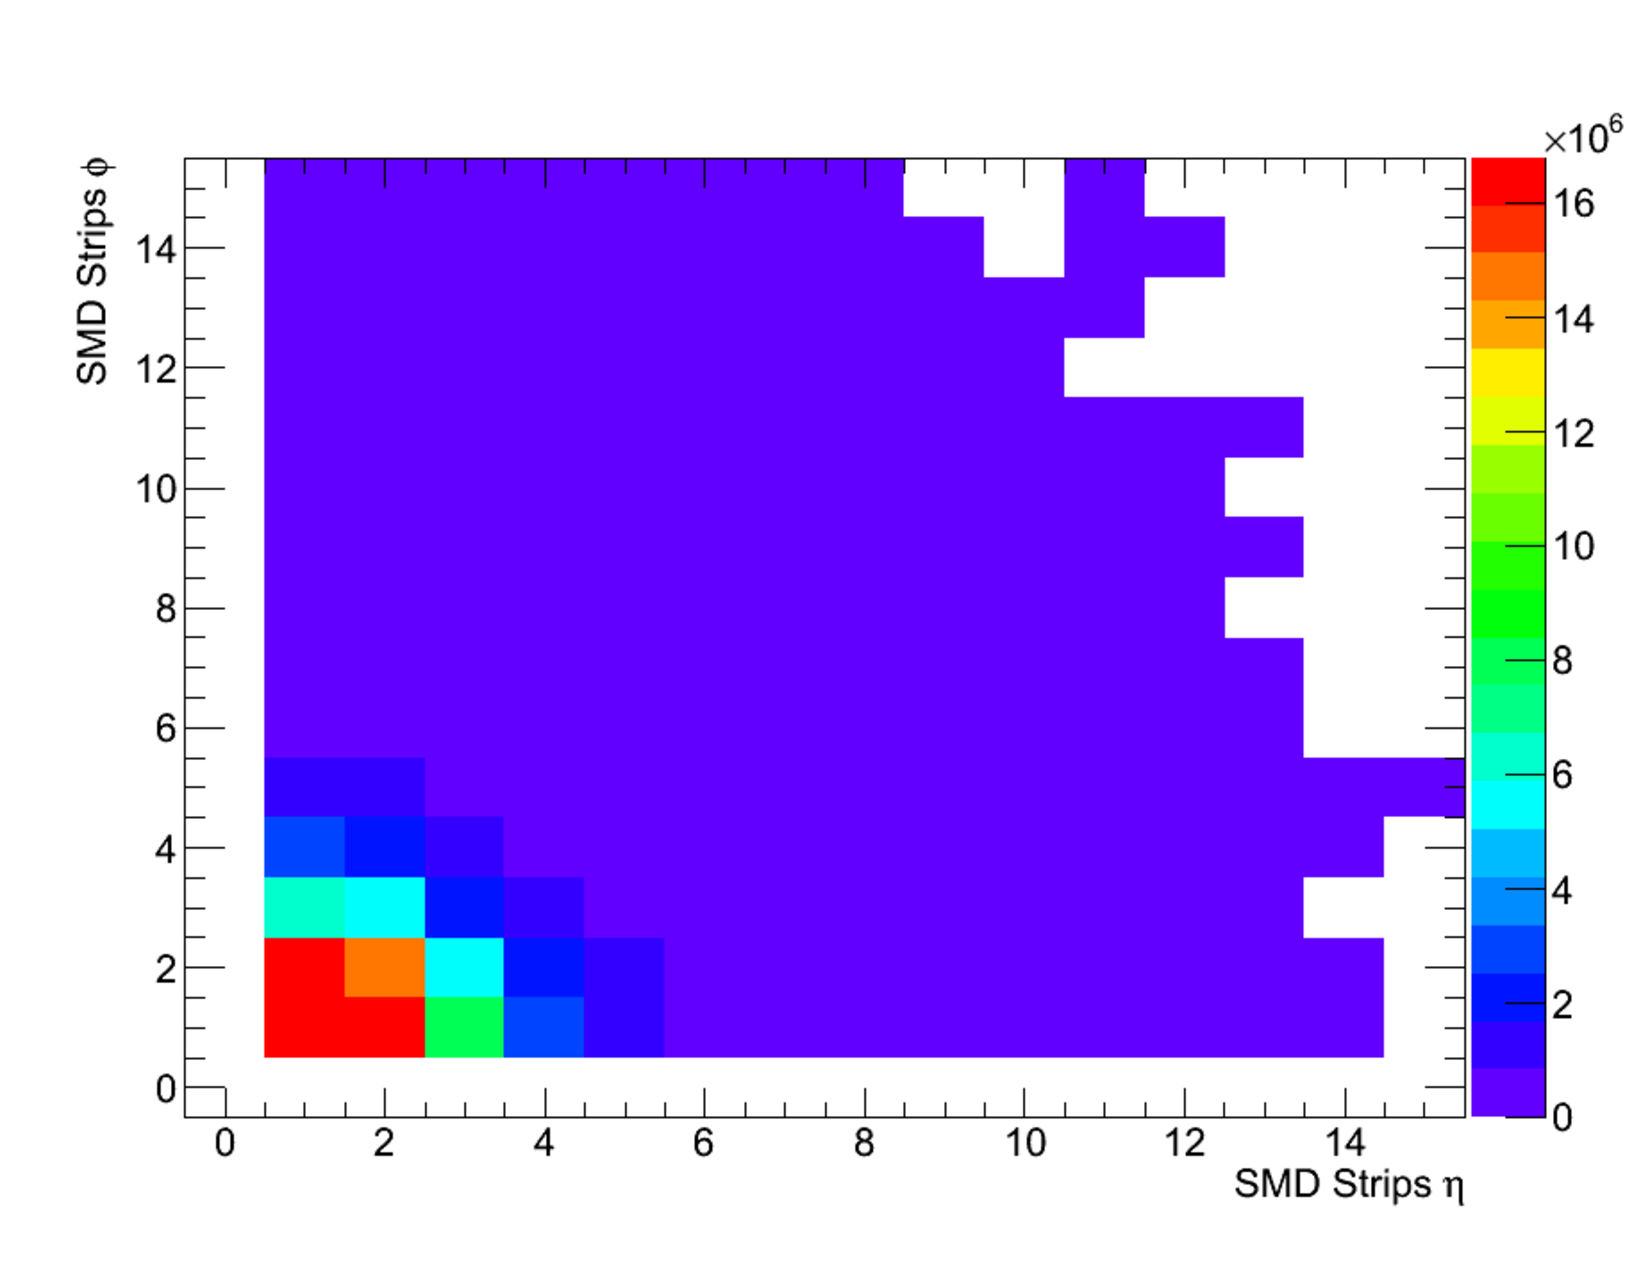
\includegraphics[width=\textwidth]{Plots/NPE/SMD_h_plot.pdf}
        \caption{Hadrons}
        \label{fig:SMD_h}
    \end{subfigure}
    \begin{subfigure}{0.65\textwidth}
        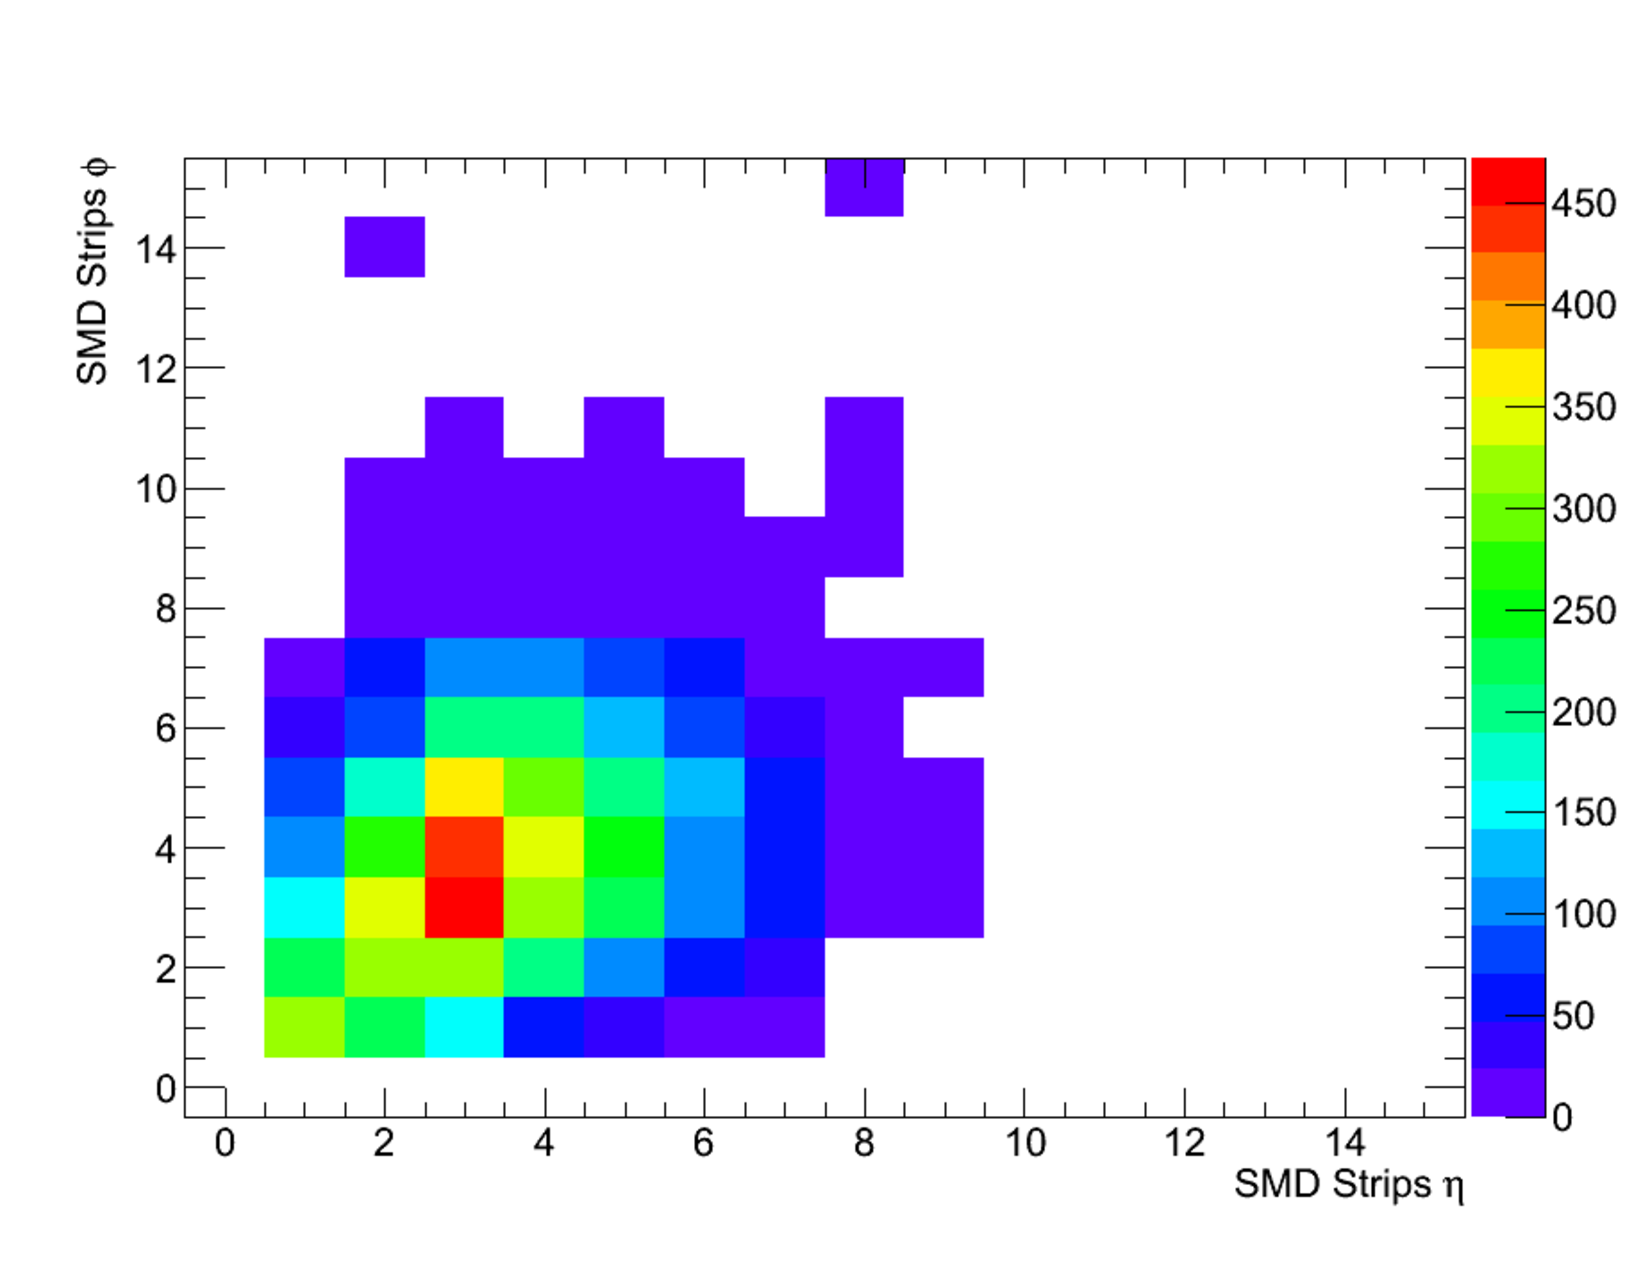
\includegraphics[width=\textwidth]{Plots/NPE/SMD_OS_plot.pdf}
        \caption{Photonic electrons}
        \label{fig:SMD_e}
    \end{subfigure}
	\end{center}
\caption[SMD Strip Hits]{SMD strip hits for hadrons and electrons. For the electron sample we take photonic electrons (a relatively pure electron sample) and remove the SMD cuts to see the number of strip hits in each direction.}
\label{fig:SMDstrips}
\end{figure}

We can also select for electrons by looking at how much energy tracks deposit into the BEMC towers. The towers of the BEMC are around 20 radiation lengths thick meaning electrons will shower and deposit all of their energy within the tower. Hadrons or muons are not likely to develop full showers in the tower and we can use this to pick out electrons. We are interested in the $E/p$ ratio for tracks hitting the BEMC. For high $p_T$ electrons, they will deposit all of their energy $E$ in the tower and since we are at high $p_T$ ($> 2$ GeV/c) we also expect that $E \approx pc$. Thus for electrons we should see $E/p \approx 1$ (ignoring factors of c). Figure~\ref{fig:EOP} shows the $E/p$ shape for electrons before applying $E/p$ cuts and hadrons. Peak is seen for electrons around 1, we set the cut for electrons to be .5 $\leq E/p \leq$ 1.7.

\begin{figure}[htbp]
\begin{center}
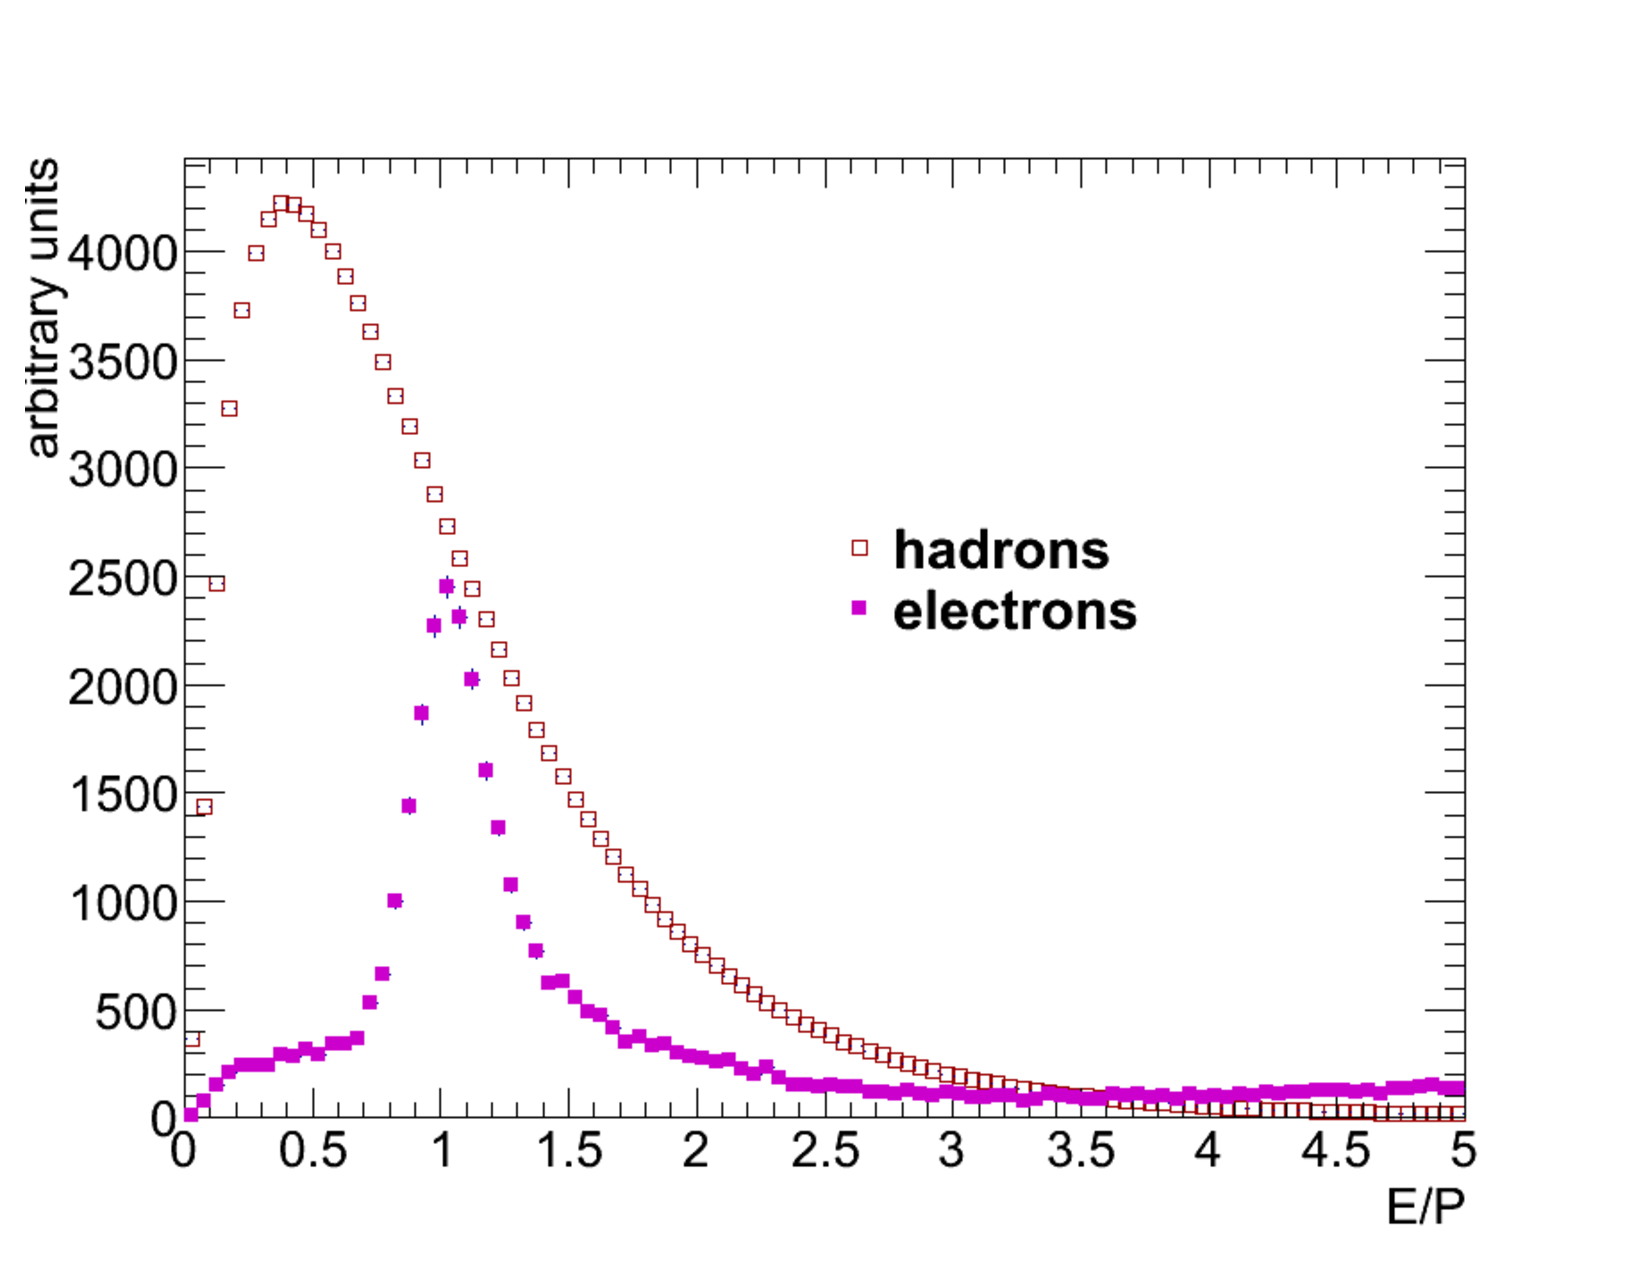
\includegraphics[scale=.65]{Plots/NPE/EOP_plot.pdf}
\end{center}
\caption[$E/p$ in BEMC]{$E/p$ for points in the BEMC for electrons (without $E/p$ cut applied) and hadrons. Scale is arbitrary to show both cases. Electron cut is set .5 $\leq E/p \leq$ 1.7.}
\label{fig:EOP}
\end{figure}

Table~\ref{tab:ecuts} summarizes the electron cuts used so far, for the most part these cuts are applied to all tracks equally and do not depend on the track $p_T$ (the ADC0 cuts being and event-by-event exception). In the next section we will show the $n\sigma_e$ cuts which will depend on the track $p_{T}$ and then later we will look at the overall electron purity that these cuts give to our inclusive sample.

\begin{table}
\centering
\begin{tabular}{|c|c|}
\hline
Variable            & Cut \\
\hline
Track Type    & $<.5$ (Primary) \\
\hline
$\eta$          & $\in(-.7, .7)$ \\
\hline
Charge               & $\pm 1$ \\
\hline
ADC0          & $\geq$205,270,325,425 (NPE11/15/18/25) \\
\hline
SMD $\phi$ Strips        & $\geq 2$ \\
\hline
SMD $\eta$ Strips        & $\geq 2$ \\
\hline
 $E/p$        & $\in(.5, 1.7)$ \\
\hline
DCA Global        & $\leq 1.5$ \\
\hline
BEMC $\Delta\phi$        & $\in(-.013, .013)$ \\
\hline
BEMC $\Delta Z$ ($\eta > 0$)    & $\in(-2.5, 1.1)$ \\
\hline
BEMC $\Delta Z$ ($\eta < 0$)    & $\in(-1.5, 1.9)$ \\
\hline
\end{tabular}
\caption[Electron Cuts]{Track level electron cuts, excluding $n\sigma_e$, cuts for Au+Au collisions.}
\label{tab:ecuts}
\end{table}

\subsection{TPC Cuts}

The only remaining cuts are those for ionization energy loss in the TPC. The energy loss varies significantly for different particle species as a function of the particle's momentum. Since we are looking for electrons the cuts we will be applying to tracks are based on the calculated $n\sigma_e$ as defined in Equation~\ref{eq:nsigmae}. For electrons $n\sigma_e$ should be distributed around 0, but for negative values of $n\sigma_e$ the electrons are overwhelmed by contamination from hadrons. We keep these cuts the same as they are in the run 10 NPE analysis, but they could be further tuned to improve electron purity and efficiency. Table~\ref{tab:nsigma} summarizes the $n\sigma_e$ cuts used for electron identification. The cuts are the same for both Au+Au and p+p data.

\begin{table}
\centering
\begin{tabular}{|c|c|}
\hline
$p_T$ Range            & $n\sigma_e$ Cut \\
\hline
1.0 GeV/c $< p_T <$ 2.0 GeV/c   & -1.25 $< n\sigma_e <$ 2\\
\hline
2.0 GeV/c $< p_T <$ 4.0 GeV/c   & -0.75 $< n\sigma_e <$ 2\\
\hline
4.0 GeV/c $< p_T <$ 6.0 GeV/c   & -0.25 $< n\sigma_e <$ 2\\
\hline
6.0 GeV/c $< p_T <$ 7.0 GeV/c   & 0.25 $< n\sigma_e <$ 2\\
\hline
7.0 GeV/c $< p_T <$ 8.0 GeV/c   & 0.25 $< n\sigma_e <$ 2\\
\hline
8.0 GeV/c $< p_T <$ 10.0 GeV/c   & 0.5 $< n\sigma_e <$ 2\\
\hline
10.0 GeV/c $< p_T <$ 12.0 GeV/c   & 0.5 $< n\sigma_e <$ 2\\
\hline
\end{tabular}
\caption[$n\sigma_e$ Cuts]{$n\sigma_e$ cuts as a function of $p_T$.}
\label{tab:nsigma}
\end{table}

\section{Electron Purity}

We will now investigate the purity of the electron sample we get from applying our electron identification cuts. To do this we will be relying on the $n\sigma_e$ distributions we have measured. First we will look at the $n\sigma_e$ distributions with all of the BEMC and track quality cuts applied. Then we will fit the peaks in $n\sigma_e$ with gaussian functions, apply the $n\sigma_e$ cuts as established in Table~\ref{tab:nsigma}, and then calculate the yields from the electron and hadron peaks. This will give us an estimate of the purity of the electron sample we will use in the NPE analysis.

\begin{figure}[htbp]
    \begin{subfigure}{0.5\textwidth}
        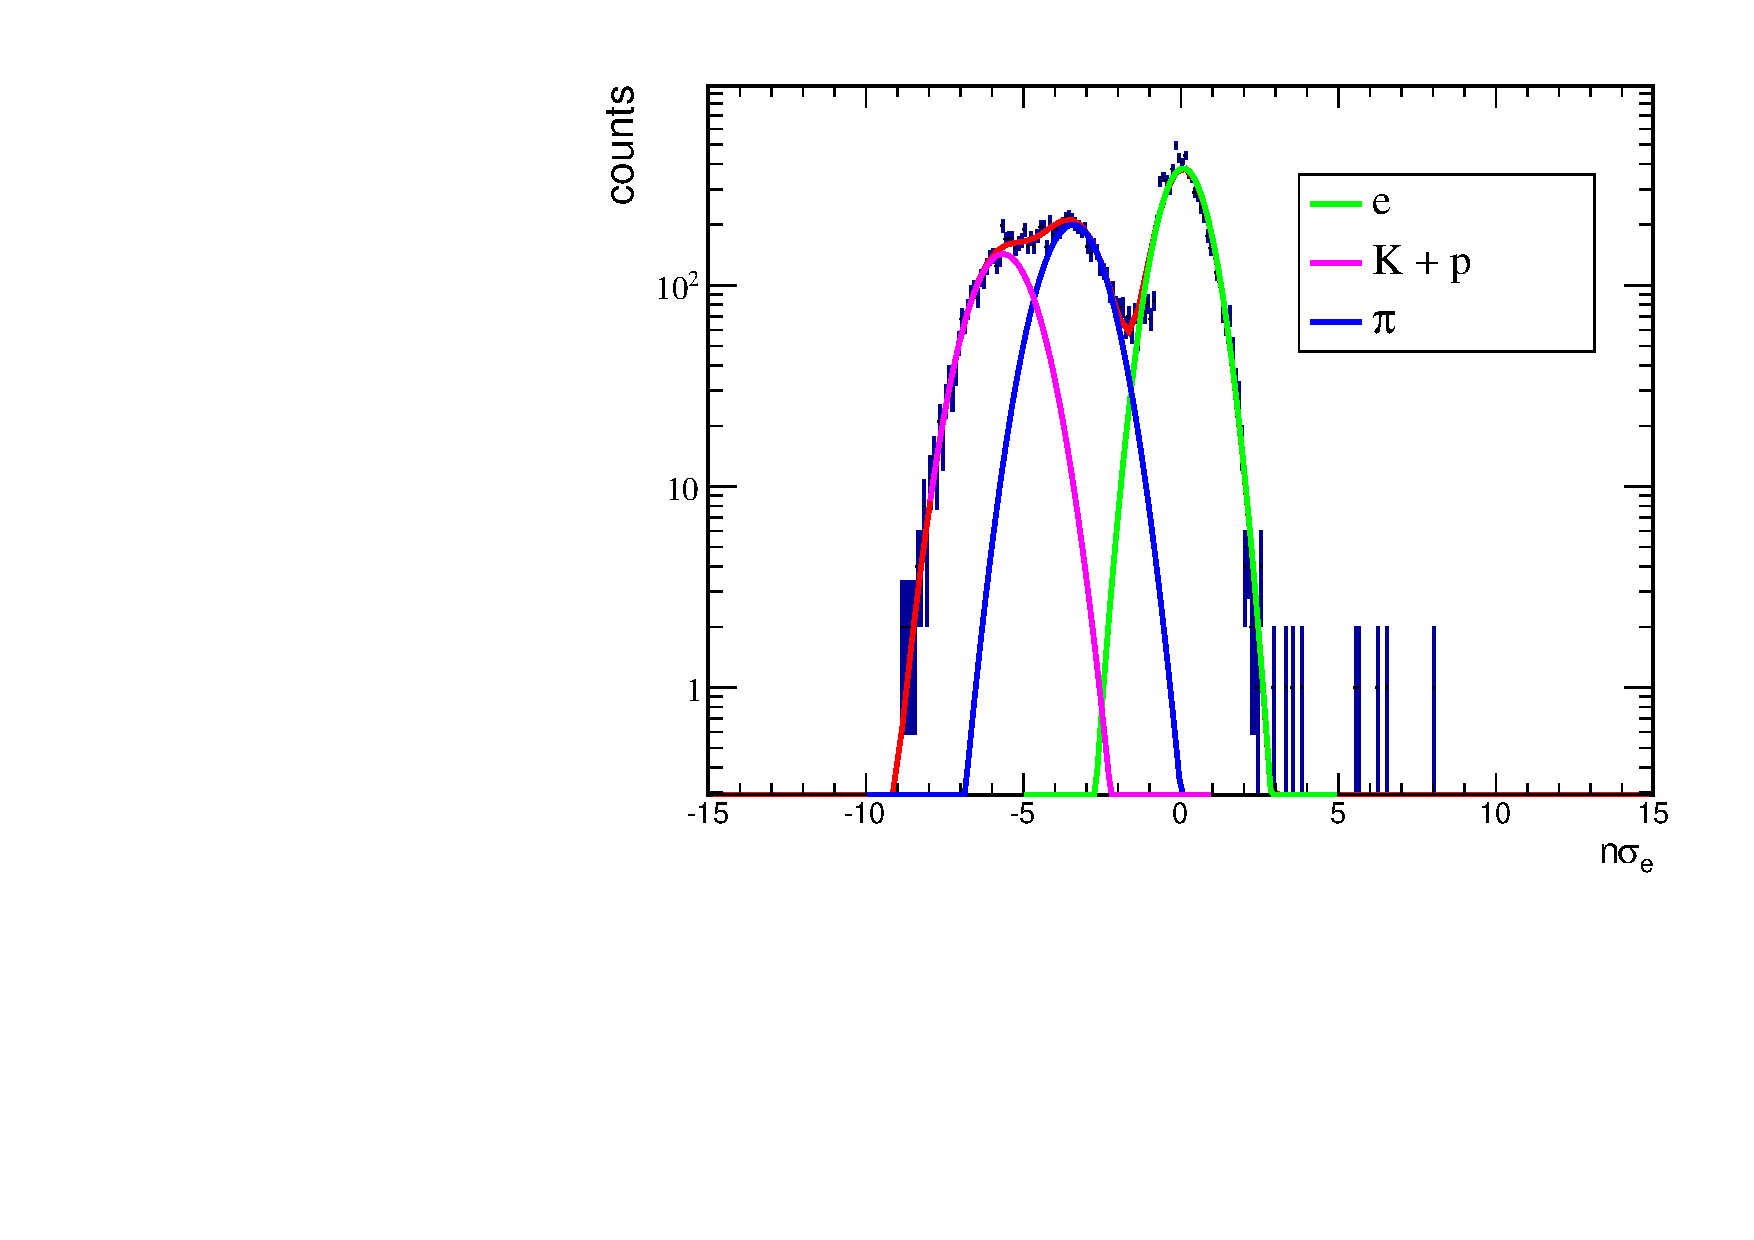
\includegraphics[width=\textwidth]{Plots/NPE/nsigmae/nsig_3_4.pdf}
        \caption{3.0 GeV/c $\leq p_{T} \leq$ 4.0 GeV/c}
        \label{fig:nsigma_3_4}
    \end{subfigure}
    \begin{subfigure}{0.5\textwidth}
        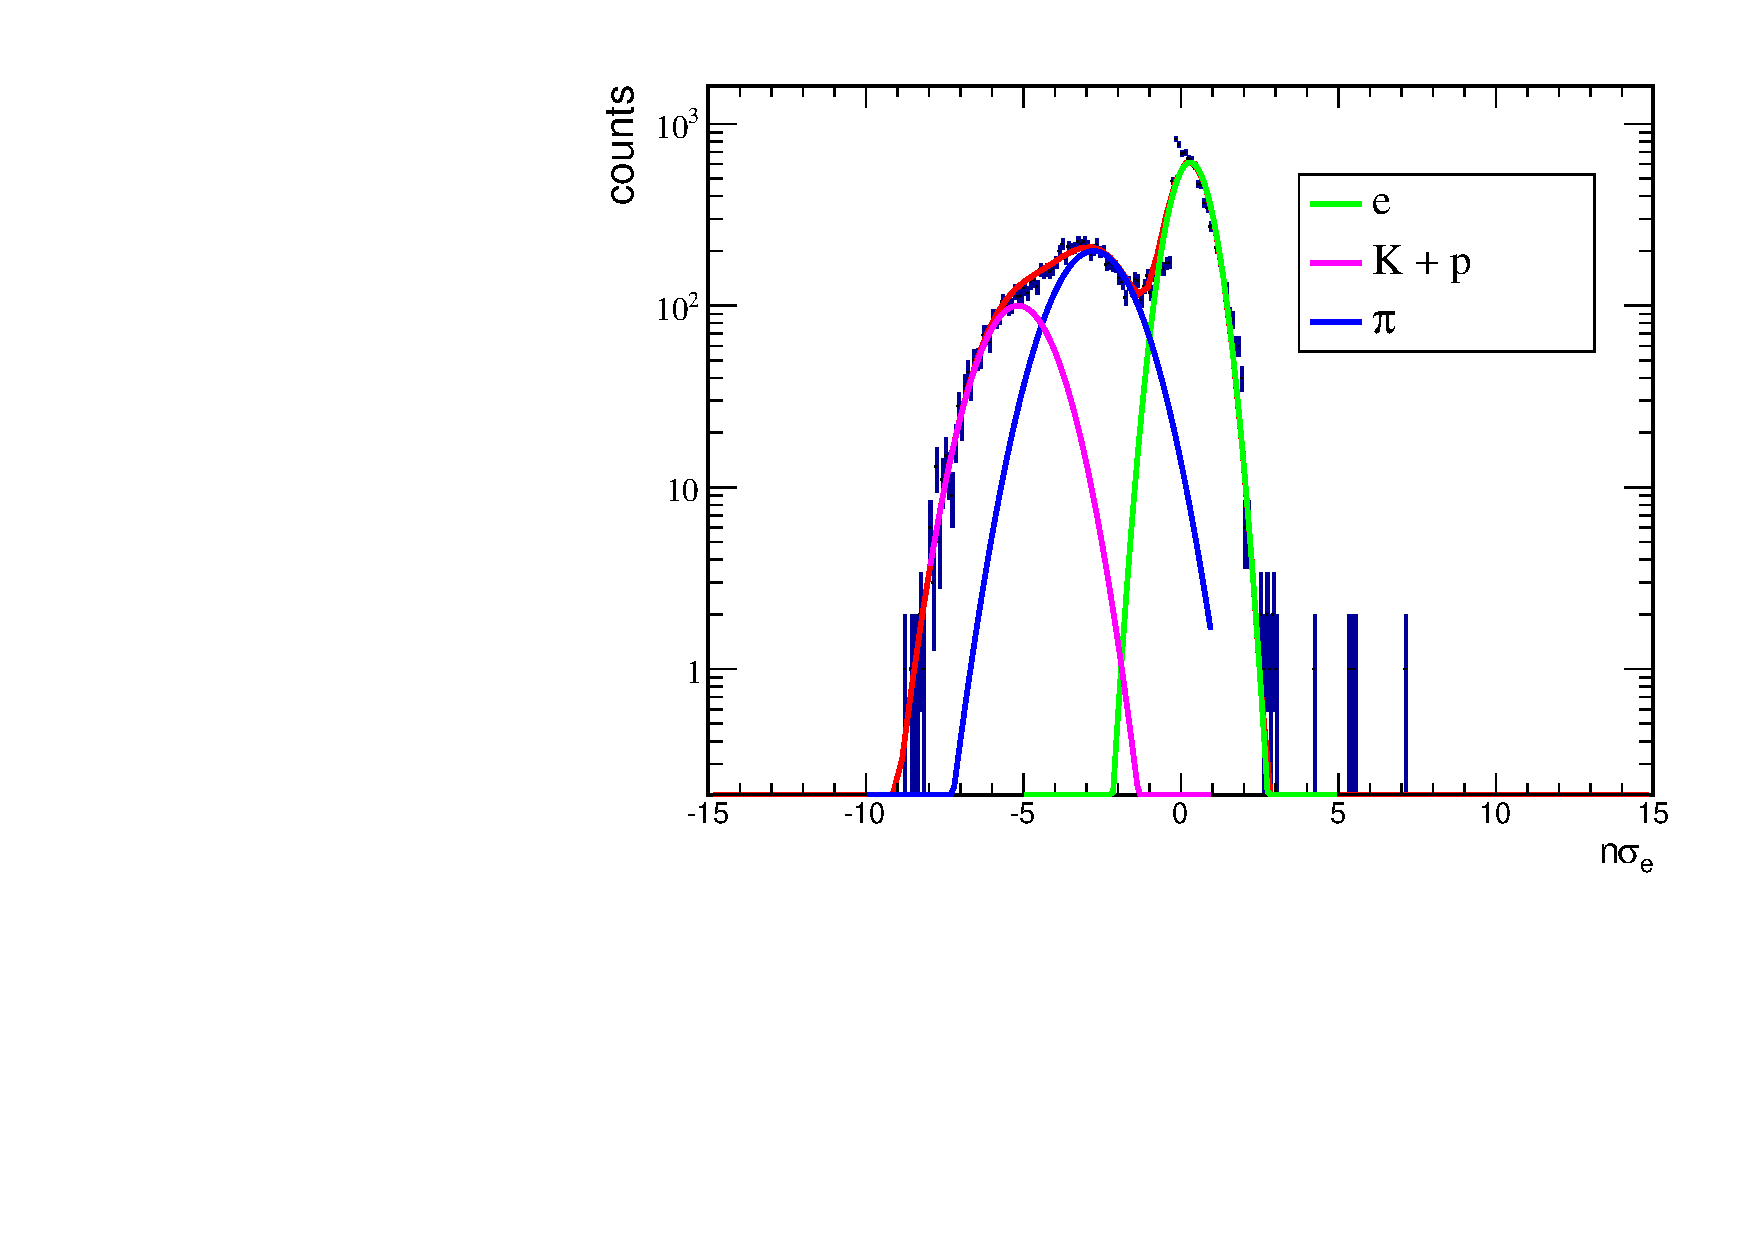
\includegraphics[width=\textwidth]{Plots/NPE/nsigmae/nsig_4_5.pdf}
        \caption{4.0 GeV/c $\leq p_{T} \leq$ 5.0 GeV/c}
        \label{fig:nsigma_4_5}
    \end{subfigure}
    \begin{subfigure}{0.5\textwidth}
        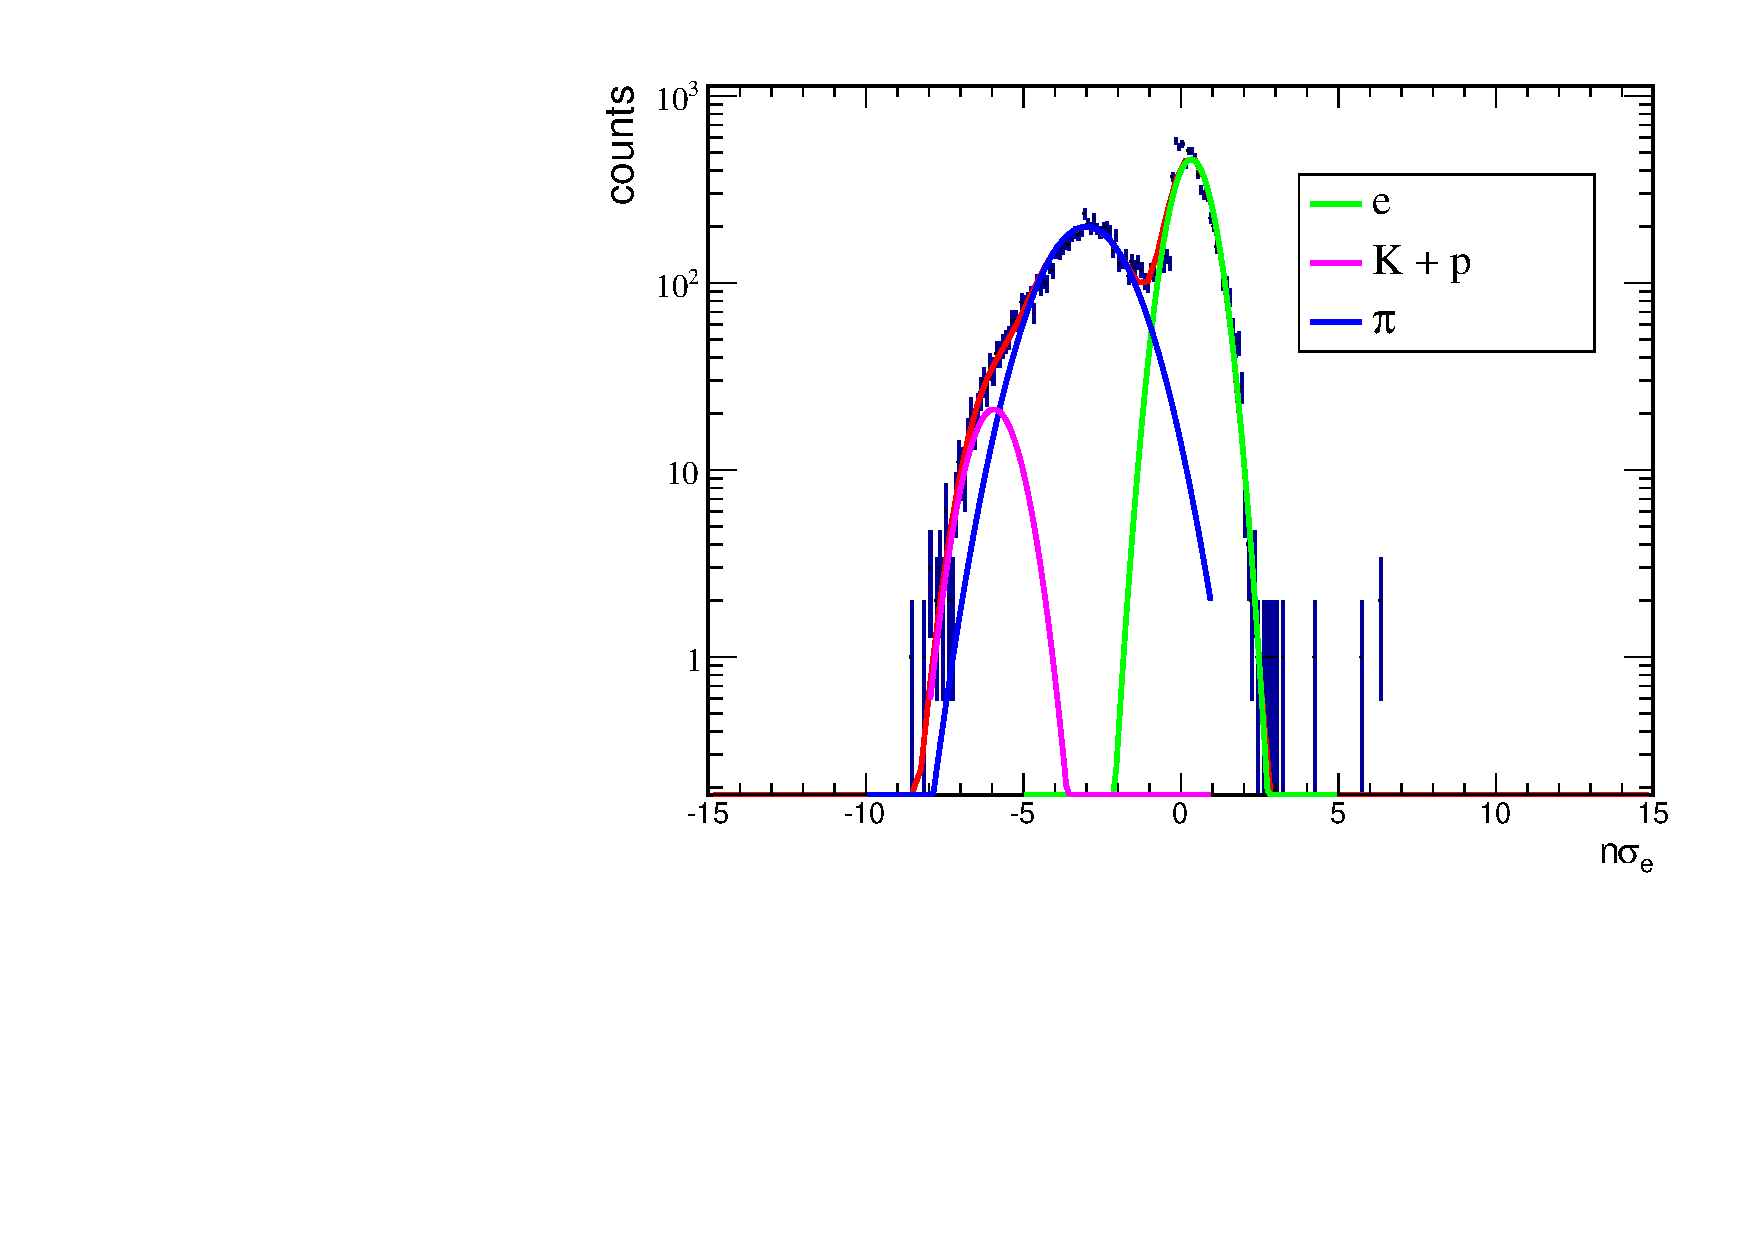
\includegraphics[width=\textwidth]{Plots/NPE/nsigmae/nsig_5_6.pdf}
        \caption{5.0 GeV/c $\leq p_{T} \leq$ 6.0 GeV/c}
        \label{fig:nsigma_5_6}
    \end{subfigure}
    \begin{subfigure}{0.5\textwidth}
        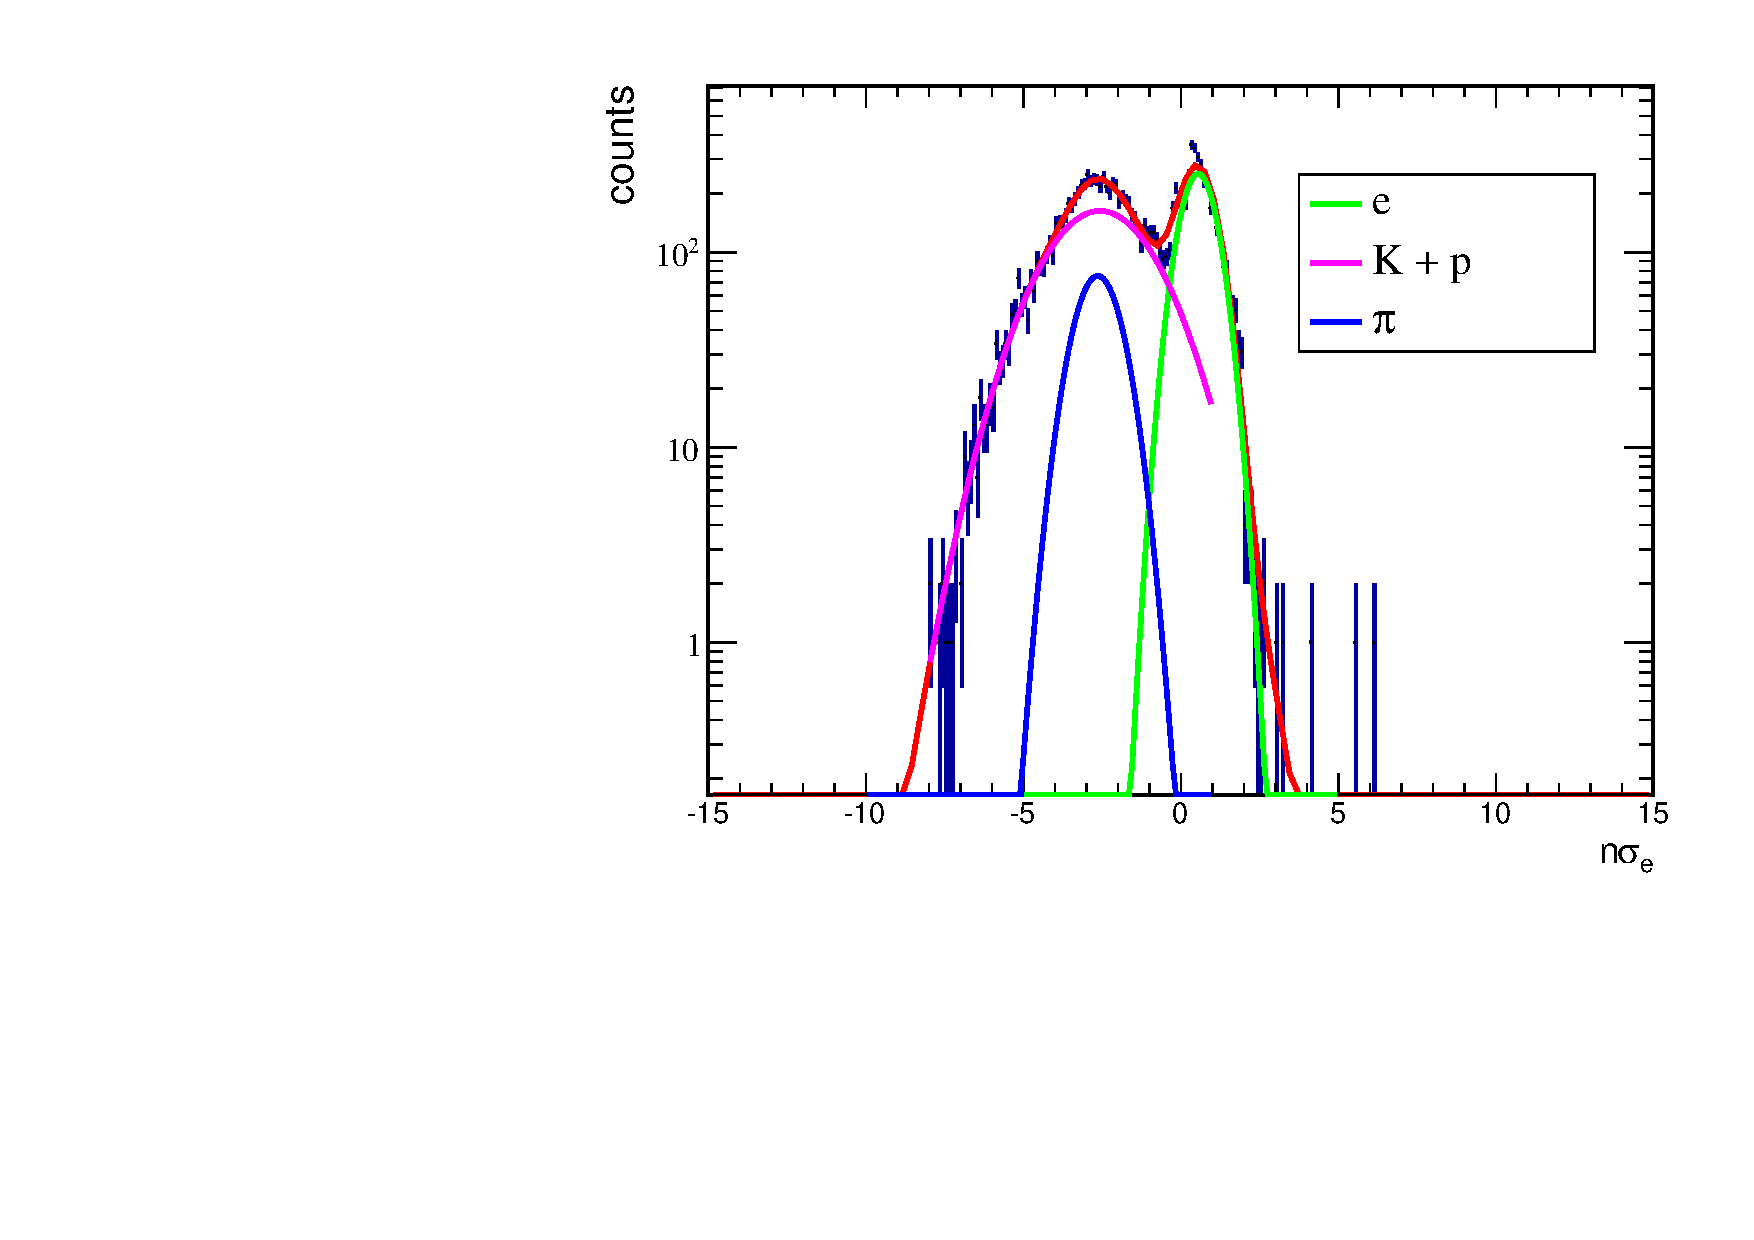
\includegraphics[width=\textwidth]{Plots/NPE/nsigmae/nsig_6_8.pdf}
        \caption{6.0 GeV/c $\leq p_{T} \leq$ 8.0 GeV/c}
        \label{fig:nsigma_6_8}
    \end{subfigure}
\caption[Fits of $n\sigma_e$]{Fits to the $n\sigma_e$ distributions for primary electron candidates (particles that pass all electron cuts excluding the $n\sigma_e$ cut) as a function of particle $p_T$. }
\label{fig:nsigma_fits}
\end{figure}

Figure~\ref{fig:nsigma_fits} shows the $n\sigma_e$ distributions as well as the fit functions. Each distribution was fit with three gaussian functions, one each for $e^{\pm}$, $\pi^{\pm}$, and a final function for $K^{\pm} + p^{\pm}$ combined. To estimate the purity we take the parameters (height, $\mu$, $\sigma$) gaussian component of the electron and hadron peaks. Then we integrate the peaks over the range specified by the $n\sigma_e$ cuts. The purity is then the fraction of the total yield that comes from the electron peak. Table~\ref{tab:purity} lists the purities obtained by this method for a range of electron $p_T$. Below 6 GeV/c the purity is quite high between 96\% and 100\%, it begins to drop for higher $p_T$ due to narrowing and shifting of the electron peak as well as closer merging of the hadron peaks with the electrons. The peak shape is biased by the fact that we only select events with high $p_T$ tracks and $n\sigma_e$ within certain values. This causes the peaks to have non-gaussian features and prevents us from taking the purities obtained at face value. However, in this analysis we will not directly need the electron purity unlike if we were looking at NPE $v_2$. We will be normalizing our observations per trigger particle, so we only need to look at purity to estimate the contribution of hadron contamination in the NPE sample when we construct NPE-h correlations.  

\begin{table}
\centering
\begin{tabular}{|c|c|}
\hline
Electron $p_T$         & Purity \\
\hline
3.0 GeV/c $< p_T <$ 4.0 GeV/c   & 99.8\% \\
\hline
4.0 GeV/c $< p_T <$ 5.0 GeV/c   & 97.0\% \\
\hline
5.0 GeV/c $< p_T <$ 6.0 GeV/c   & 96.1\% \\
\hline
6.0 GeV/c $< p_T <$ 8.0 GeV/c   & 79.6\% \\
\hline
\end{tabular}
\caption[Electron Purity]{Purity of electrons obtained from fits to $n\sigma_e$.}
\label{tab:purity}
\end{table}

\section{Photonic Electron Identification}

The main background to electrons from the decay of heavy flavor mesons comes from photon conversions in the detector and Dalitz decay of $\pi$ and $\eta$ mesons. Collectively we refer to these background electrons as \textit{photonic electrons}, and in this section we will summarize how we remove them from our electron sample. When the electrons are produced by these background processes they come in $e^{+}e^{-}$ pairs. To tell whether an electron is of photonic origin we search through the tracks in the event and try to find its partner.

When searching for the partner electron we use very relaxed cuts. We search through all global tracks (rather than primary) within a pseudorapidty of -1.3 $\leq \eta \leq$ 1.3. To cut out hadrons we require that -3 $\leq n\sigma_e \leq$ 3. Tracks from photonic background will be very close together in the detector and will have a small opening angle. We apply cuts on the pairwise DCA of the two tracks, requiring the DCA be less than 1.0 cm. Also the opening angle between the tracks should be small, we want the total angle $\Theta <$ 0.05 and the azimuthal angle $\phi < $ 0.1. Table~\ref{tab:pe_cuts} summarizes the track cuts and pairing criteria for reconstructing photonic electrons. The partner for a photonic electron must have opposite charge to the primary track. We look for both opposite-sign as well as like-sign pairs. The like sign pairs which satisfy the photonic partner cuts let us estimate the number of photonic electrons that are misidentified due to combinatorial pairing of tracks.

\begin{figure}[htbp]
	\begin{center}
    \begin{subfigure}{0.65\textwidth}
        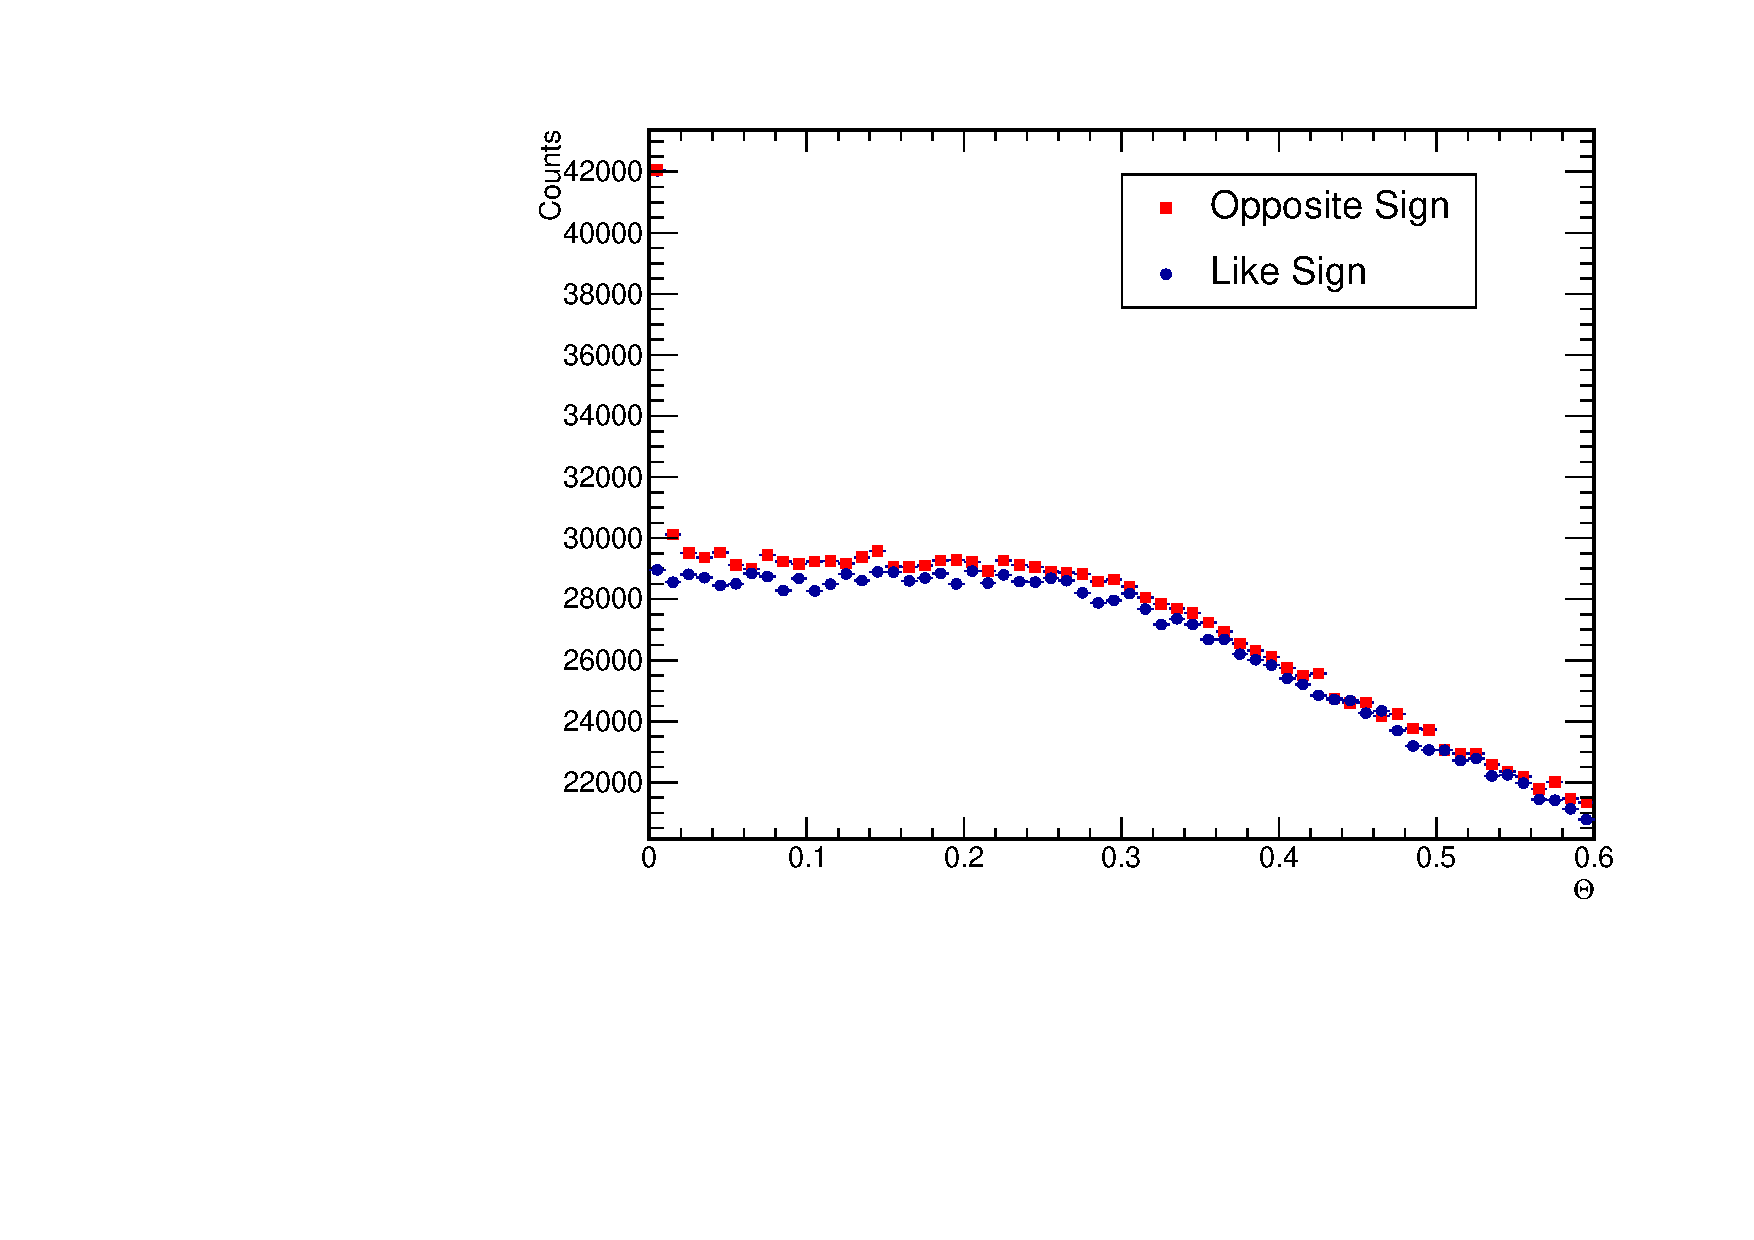
\includegraphics[width=\textwidth]{Plots/NPE/Theta_OS_LS.pdf}
        \caption{$\eta >$ 0}
        \label{fig:PE_Theta}
    \end{subfigure}
    \begin{subfigure}{0.65\textwidth}
        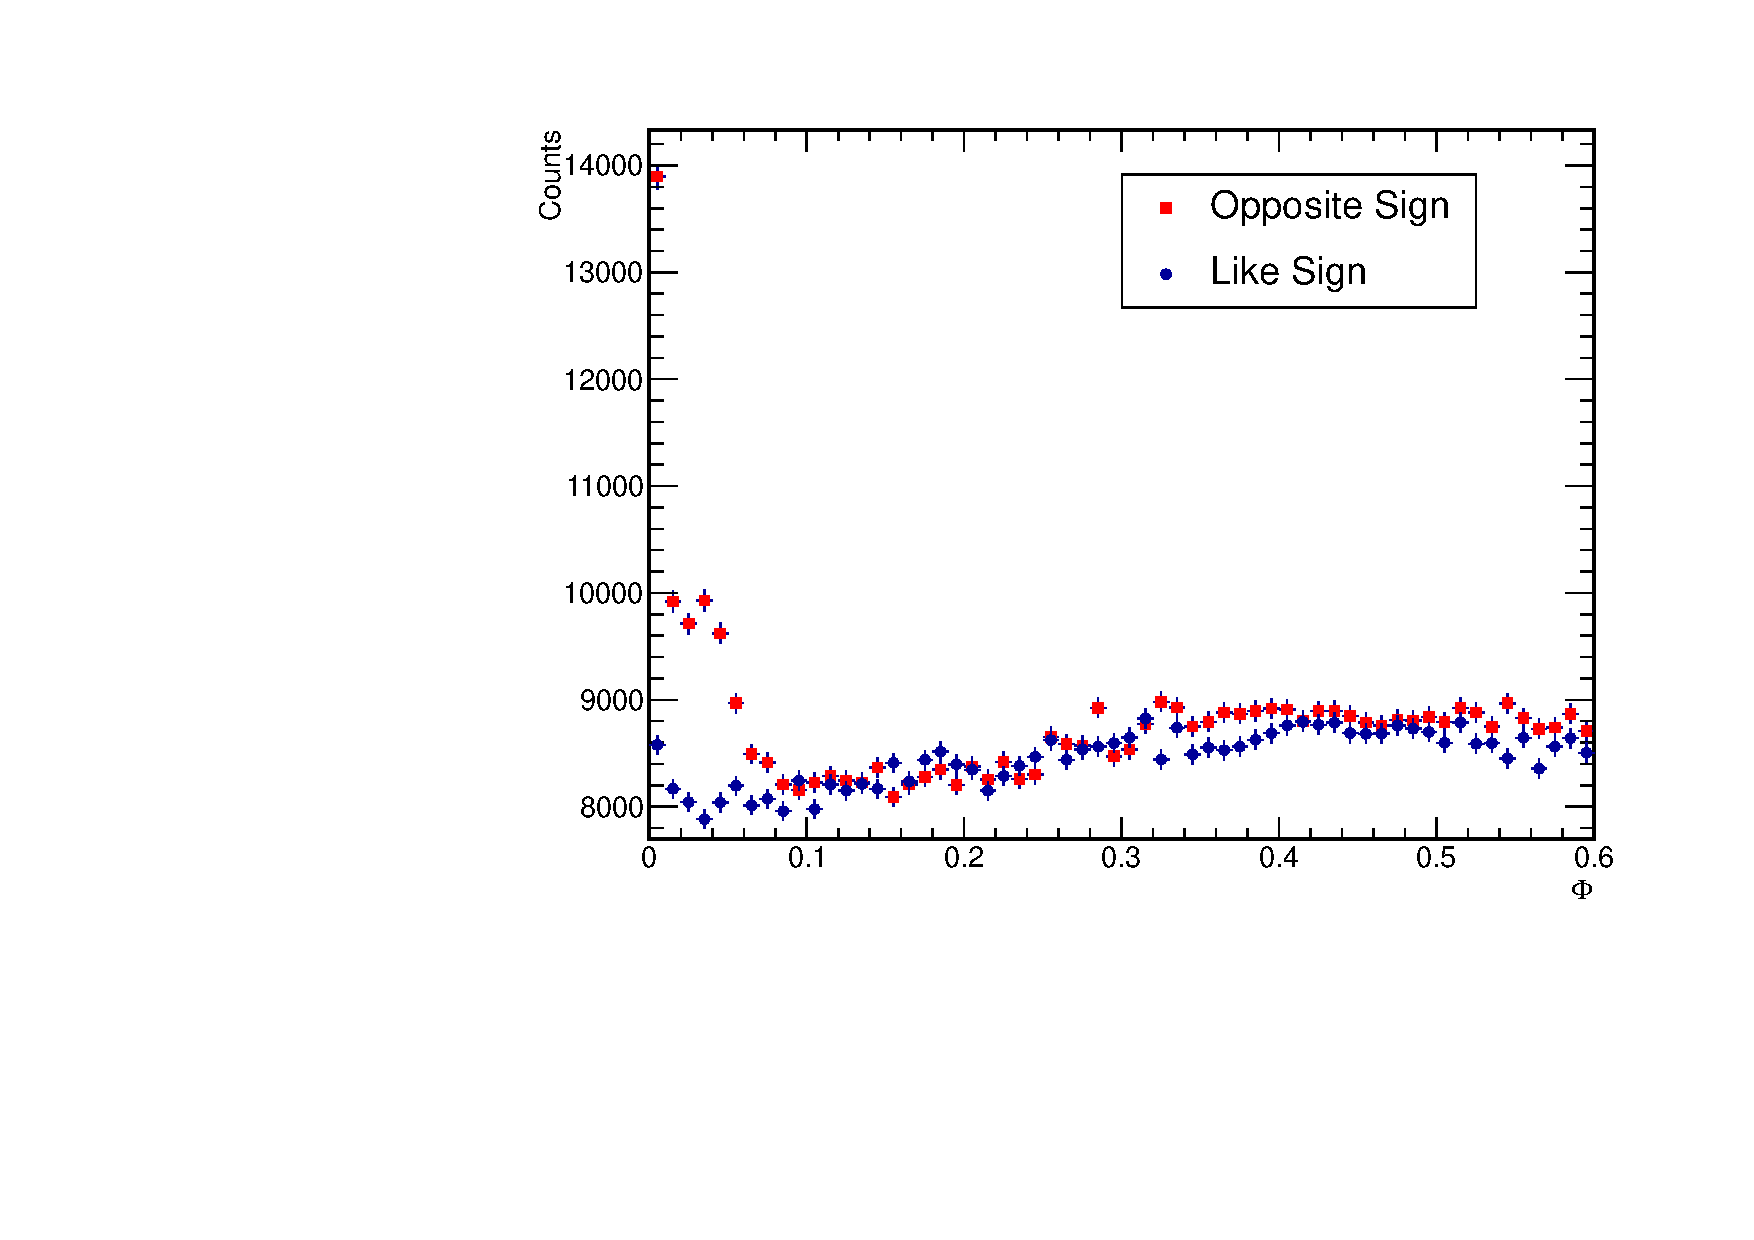
\includegraphics[width=\textwidth]{Plots/NPE/Phi_OS_LS.pdf}
        \caption{$\eta <$ 0}
        \label{fig:PE_Phi}
    \end{subfigure}
	\end{center}
\caption[Angle Cuts for Phot. Electrons]{Angle cuts for partner tracks used to recontstruct photonic electrons.}
\label{fig:PE_angle}
\end{figure}

\begin{table}
\centering
\begin{tabular}{|c|c|}
\hline
Variable         & Cuts \\
\hline
TrackType   & Global \\
\hline
$\eta$   & $\in(-1.3,1.3)$ \\
\hline
$p_T$   & $> 0.3$ GeV/c \\
\hline
Pair DCA  & $< 1.0$ cm \\
\hline
Pair $\Theta$   & $< 0.05$ \\
\hline
Pair $\phi$   & $< 0.10$ \\
\hline
2D Invariant Mass   & $< 0.10$ GeV/$c^2$ \\
\hline
\end{tabular}
\caption[Photonic Electron Cuts]{Cuts used for partner tracks and for identifying photonic electrons.}
\label{tab:pe_cuts}
\end{table}

For photonic electrons we expect the pair of particles to have a low invariant mass (exactly 0 for photon conversions and $< .1$ GeV/$c^2$ for Dalitz decays). However the measurement of the invariant mass is degraded by the finite tracking resolution of the TPC. Reconstructed TPC tracks form helices in the detector volume. The resolution of the TPC effectively means that the helices can shift around relative to each other. Due to this effect, there is a large uncertainty in the location of the secondary vertex where the electrons have their minimum DCA. This causes an uncertainty in the opening angle between the tracks and smears out the invariant mass distribution of the pairs. To correct this we instead consider the 2D invariant mass. The tracks are rotated into the same plane before calculating the mass. The cutoff for photonic electrons is that this 2D invariant mass be below .10 GeV/$c^2$. Figure~\ref{fig:2DInvMass} shows the 2D invariant mass distribution. The 3D invariant mass is not used in identifying photonic electrons but is plotted in Figure~\ref{fig:InvMass}. The peak near 0 is from photon conversions while the peak at .05 GeV/$c^2$ comes from the Dalitz decays. The Dalitz decay is a three body decay and thus the missing photon causes the mass peak to be smeared.

Clearly just pairing up all tracks to look for photonic electrons will not guarantee that we remove all of the background. It is possible for the partner track to be outside of our acceptance or otherwise fail to pass the photonic electron cuts. We will quantify how much background we miss by the parameter $\epsilon_\gamma$, the photonic reconstruction efficiency, which is essentially the fraction of all photonic electrons we are able to reconstruct from searching for partner tracks. The next section will discuss how $\epsilon_\gamma$ is calculated.

\begin{figure}[htbp]
\begin{center}
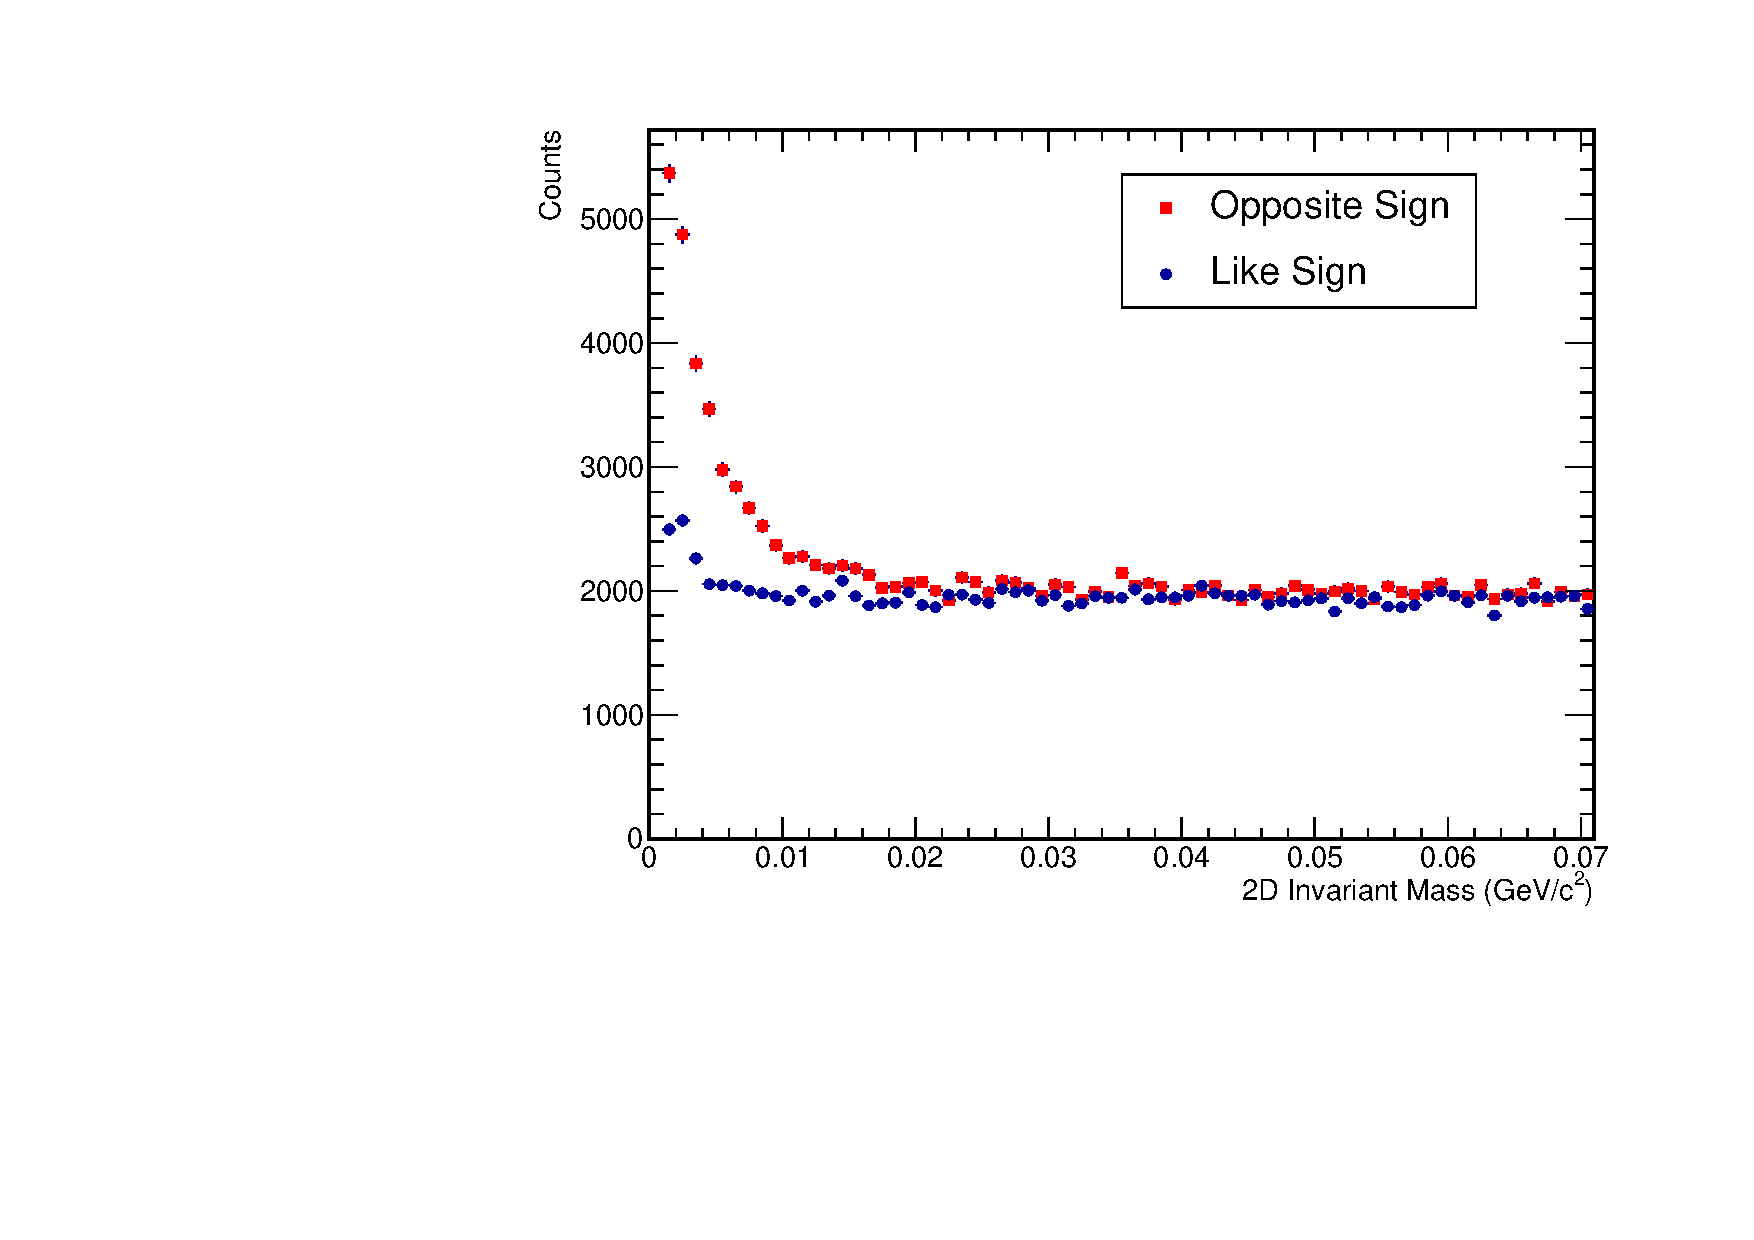
\includegraphics[scale=.8]{Plots/NPE/2DInvMass_OS_LS.pdf}
\end{center}
\caption[2D Invariant Mass]{2D invariant mass for opposite sign and same sign pairs. For photonic electron identification we require that $m_{2D} <$ 0.10 GeV/$c^2$.}
\label{fig:2DInvMass}
\end{figure}

\begin{figure}[htbp]
\begin{center}
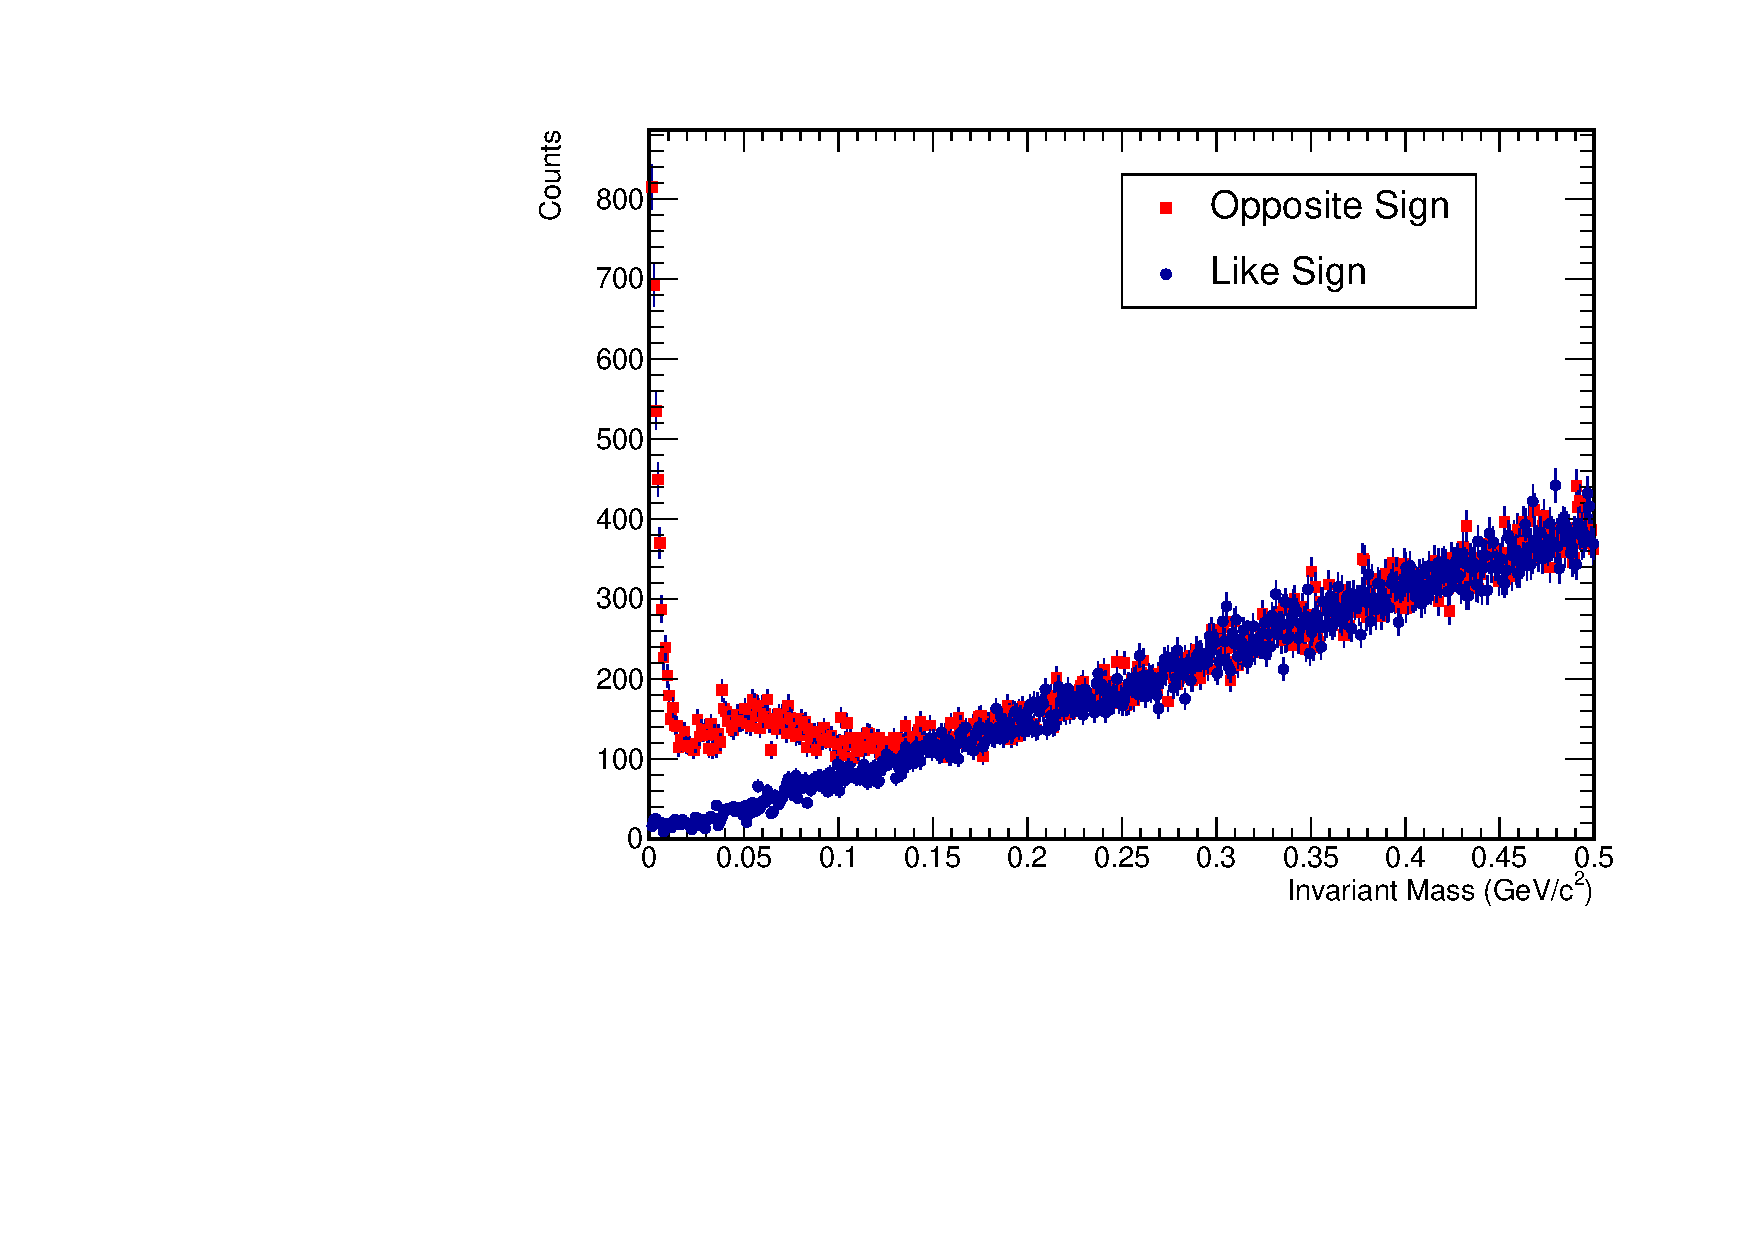
\includegraphics[scale=.8]{Plots/NPE/InvMass_OS_LS.pdf}
\end{center}
\caption[Invariant Mass]{Invariant mass distribution for pairs of tracks. Opposite sign pairs show low mass excess which corresponds to the photonic electrons.}
\label{fig:InvMass}
\end{figure}

\section{Photonic Electron Reconstruction Efficiency}
